\documentclass[11pt]{article}
\usepackage[margin=1in]{geometry}
\usepackage[T1]{fontenc}
\usepackage[utf8]{inputenc}
\usepackage{lmodern,microtype,amsmath,amssymb,graphicx,booktabs,longtable,pdflscape}
\usepackage[round,authoryear]{natbib}
\usepackage[hidelinks]{hyperref}
\usepackage{caption}
\captionsetup{font=small,labelfont=bf}
\setlength{\parskip}{.35em}
\setlength{\parindent}{1em}
\setlength{\tabcolsep}{4pt}
\newcommand{\valueof}[1]{\ifcsname value:#1\endcsname\csname value:#1\endcsname\else\PackageError{oos}{Missing generated value #1}{Run make oos-paper}\fi}
\newcommand{\policy}[2]{\valueof{#1.policy.paired.#2}}
\newcommand{\pollvalue}[2]{\valueof{#1.policy.available.#2}}
\newcommand{\component}[3]{\valueof{#1.components.policy.#2.#3}}
\newcommand{\overall}[3]{\valueof{overall.#1.policy.paired.#2.#3}}
\expandafter\def\csname value:correctedoriginal.policy.available.h\endcsname{0.013}
\expandafter\def\csname value:correctedoriginal.policy.available.p\endcsname{-0.022}
\expandafter\def\csname value:correctedoriginal.policy.available.d_gender\endcsname{0.002}
\expandafter\def\csname value:correctedoriginal.policy.available.d_education\endcsname{0.010}
\expandafter\def\csname value:correctedoriginal.policy.available.d_income\endcsname{0.002}
\expandafter\def\csname value:correctedoriginal.policy.available.d_combined\endcsname{0.013}
\expandafter\def\csname value:correctedoriginal.policy.available.p_absolute\endcsname{0.009}
\expandafter\def\csname value:correctedoriginal.policy.paired.h\endcsname{0.012}
\expandafter\def\csname value:correctedoriginal.policy.paired.p\endcsname{-0.022}
\expandafter\def\csname value:correctedoriginal.policy.paired.d_gender\endcsname{0.002}
\expandafter\def\csname value:correctedoriginal.policy.paired.d_education\endcsname{0.011}
\expandafter\def\csname value:correctedoriginal.policy.paired.d_income\endcsname{0.003}
\expandafter\def\csname value:correctedoriginal.policy.paired.d_combined\endcsname{0.014}
\expandafter\def\csname value:correctedoriginal.policy.paired.p_absolute\endcsname{0.008}
\expandafter\def\csname value:a1r2019.policy.available.h\endcsname{0.035}
\expandafter\def\csname value:a1r2019.policy.available.p\endcsname{0.013}
\expandafter\def\csname value:a1r2019.policy.available.d_gender\endcsname{0.006}
\expandafter\def\csname value:a1r2019.policy.available.p_absolute\endcsname{0.045}
\expandafter\def\csname value:a1r2019.policy.paired.h\endcsname{0.034}
\expandafter\def\csname value:a1r2019.policy.paired.p\endcsname{0.014}
\expandafter\def\csname value:a1r2019.policy.paired.d_gender\endcsname{0.007}
\expandafter\def\csname value:a1r2019.policy.paired.p_absolute\endcsname{0.047}
\expandafter\def\csname value:ourbudgetoureconomy.policy.available.h\endcsname{0.017}
\expandafter\def\csname value:ourbudgetoureconomy.policy.available.p\endcsname{-0.017}
\expandafter\def\csname value:ourbudgetoureconomy.policy.available.d_gender\endcsname{0.008}
\expandafter\def\csname value:ourbudgetoureconomy.policy.available.d_education\endcsname{0.005}
\expandafter\def\csname value:ourbudgetoureconomy.policy.available.d_income\endcsname{0.010}
\expandafter\def\csname value:ourbudgetoureconomy.policy.available.d_combined\endcsname{0.012}
\expandafter\def\csname value:ourbudgetoureconomy.policy.available.p_absolute\endcsname{0.038}
\expandafter\def\csname value:ourbudgetoureconomy.policy.paired.h\endcsname{0.008}
\expandafter\def\csname value:ourbudgetoureconomy.policy.paired.p\endcsname{-0.019}
\expandafter\def\csname value:ourbudgetoureconomy.policy.paired.d_gender\endcsname{0.005}
\expandafter\def\csname value:ourbudgetoureconomy.policy.paired.d_education\endcsname{0.003}
\expandafter\def\csname value:ourbudgetoureconomy.policy.paired.d_income\endcsname{0.006}
\expandafter\def\csname value:ourbudgetoureconomy.policy.paired.d_combined\endcsname{-0.004}
\expandafter\def\csname value:ourbudgetoureconomy.policy.paired.p_absolute\endcsname{0.028}
\expandafter\def\csname value:hongkongfacilitated.policy.available.h\endcsname{-0.145}
\expandafter\def\csname value:hongkongfacilitated.policy.available.p\endcsname{0.000}
\expandafter\def\csname value:hongkongfacilitated.policy.available.p_absolute\endcsname{0.000}
\expandafter\def\csname value:hongkongfacilitated.policy.paired.h\endcsname{-0.145}
\expandafter\def\csname value:hongkongfacilitated.policy.paired.p\endcsname{0.000}
\expandafter\def\csname value:hongkongfacilitated.policy.paired.p_absolute\endcsname{0.000}
\expandafter\def\csname value:hongkongcasual.policy.available.h\endcsname{-0.040}
\expandafter\def\csname value:hongkongcasual.policy.available.p_absolute\endcsname{0.033}
\expandafter\def\csname value:hongkongcasual.policy.paired.h\endcsname{-0.040}
\expandafter\def\csname value:hongkongcasual.policy.paired.p_absolute\endcsname{0.033}
\expandafter\def\csname value:tanzania.policy.available.h\endcsname{-0.006}
\expandafter\def\csname value:tanzania.policy.available.p\endcsname{-0.037}
\expandafter\def\csname value:tanzania.policy.available.d_gender\endcsname{-0.008}
\expandafter\def\csname value:tanzania.policy.available.p_absolute\endcsname{-0.006}
\expandafter\def\csname value:tanzania.policy.paired.h\endcsname{-0.005}
\expandafter\def\csname value:tanzania.policy.paired.p\endcsname{-0.038}
\expandafter\def\csname value:tanzania.policy.paired.d_gender\endcsname{-0.005}
\expandafter\def\csname value:tanzania.policy.paired.p_absolute\endcsname{-0.008}
\expandafter\def\csname value:a1rclimate.climate_belief.available.h\endcsname{0.044}
\expandafter\def\csname value:a1rclimate.climate_belief.available.p\endcsname{0.044}
\expandafter\def\csname value:a1rclimate.climate_belief.available.d_gender\endcsname{0.002}
\expandafter\def\csname value:a1rclimate.climate_belief.available.d_education\endcsname{0.016}
\expandafter\def\csname value:a1rclimate.climate_belief.available.d_income\endcsname{0.008}
\expandafter\def\csname value:a1rclimate.climate_belief.available.d_combined\endcsname{0.013}
\expandafter\def\csname value:a1rclimate.climate_belief.available.p_absolute\endcsname{0.046}
\expandafter\def\csname value:a1rclimate.climate_belief.paired.h\endcsname{0.044}
\expandafter\def\csname value:a1rclimate.climate_belief.paired.p\endcsname{0.045}
\expandafter\def\csname value:a1rclimate.climate_belief.paired.d_gender\endcsname{0.001}
\expandafter\def\csname value:a1rclimate.climate_belief.paired.d_education\endcsname{0.019}
\expandafter\def\csname value:a1rclimate.climate_belief.paired.d_income\endcsname{0.010}
\expandafter\def\csname value:a1rclimate.climate_belief.paired.d_combined\endcsname{0.013}
\expandafter\def\csname value:a1rclimate.climate_belief.paired.p_absolute\endcsname{0.048}
\expandafter\def\csname value:a1rclimate.environmental_concern.available.h\endcsname{0.033}
\expandafter\def\csname value:a1rclimate.environmental_concern.available.p\endcsname{0.034}
\expandafter\def\csname value:a1rclimate.environmental_concern.available.d_gender\endcsname{-0.003}
\expandafter\def\csname value:a1rclimate.environmental_concern.available.d_education\endcsname{0.019}
\expandafter\def\csname value:a1rclimate.environmental_concern.available.d_income\endcsname{0.014}
\expandafter\def\csname value:a1rclimate.environmental_concern.available.d_combined\endcsname{0.008}
\expandafter\def\csname value:a1rclimate.environmental_concern.available.p_absolute\endcsname{0.048}
\expandafter\def\csname value:a1rclimate.environmental_concern.paired.h\endcsname{0.033}
\expandafter\def\csname value:a1rclimate.environmental_concern.paired.p\endcsname{0.034}
\expandafter\def\csname value:a1rclimate.environmental_concern.paired.d_gender\endcsname{-0.003}
\expandafter\def\csname value:a1rclimate.environmental_concern.paired.d_education\endcsname{0.020}
\expandafter\def\csname value:a1rclimate.environmental_concern.paired.d_income\endcsname{0.013}
\expandafter\def\csname value:a1rclimate.environmental_concern.paired.d_combined\endcsname{0.009}
\expandafter\def\csname value:a1rclimate.environmental_concern.paired.p_absolute\endcsname{0.047}
\expandafter\def\csname value:a1rclimate.policy.available.h\endcsname{0.030}
\expandafter\def\csname value:a1rclimate.policy.available.p\endcsname{0.022}
\expandafter\def\csname value:a1rclimate.policy.available.d_gender\endcsname{0.001}
\expandafter\def\csname value:a1rclimate.policy.available.d_education\endcsname{0.010}
\expandafter\def\csname value:a1rclimate.policy.available.d_income\endcsname{0.005}
\expandafter\def\csname value:a1rclimate.policy.available.d_combined\endcsname{0.006}
\expandafter\def\csname value:a1rclimate.policy.available.p_absolute\endcsname{0.037}
\expandafter\def\csname value:a1rclimate.policy.paired.h\endcsname{0.030}
\expandafter\def\csname value:a1rclimate.policy.paired.p\endcsname{0.024}
\expandafter\def\csname value:a1rclimate.policy.paired.d_gender\endcsname{0.001}
\expandafter\def\csname value:a1rclimate.policy.paired.d_education\endcsname{0.009}
\expandafter\def\csname value:a1rclimate.policy.paired.d_income\endcsname{0.005}
\expandafter\def\csname value:a1rclimate.policy.paired.d_combined\endcsname{0.006}
\expandafter\def\csname value:a1rclimate.policy.paired.p_absolute\endcsname{0.039}
\expandafter\def\csname value:celaya.policy.available.h\endcsname{-0.015}
\expandafter\def\csname value:celaya.policy.available.p\endcsname{-0.031}
\expandafter\def\csname value:celaya.policy.available.d_gender\endcsname{-0.011}
\expandafter\def\csname value:celaya.policy.available.d_education\endcsname{-0.019}
\expandafter\def\csname value:celaya.policy.available.d_income\endcsname{-0.017}
\expandafter\def\csname value:celaya.policy.available.d_combined\endcsname{-0.014}
\expandafter\def\csname value:celaya.policy.available.p_absolute\endcsname{-0.013}
\expandafter\def\csname value:celaya.policy.paired.h\endcsname{-0.015}
\expandafter\def\csname value:celaya.policy.paired.p\endcsname{-0.031}
\expandafter\def\csname value:celaya.policy.paired.d_gender\endcsname{-0.011}
\expandafter\def\csname value:celaya.policy.paired.d_education\endcsname{-0.019}
\expandafter\def\csname value:celaya.policy.paired.d_income\endcsname{-0.017}
\expandafter\def\csname value:celaya.policy.paired.d_combined\endcsname{-0.014}
\expandafter\def\csname value:celaya.policy.paired.p_absolute\endcsname{-0.013}
\expandafter\def\csname value:uksameparty.policy.available.h\endcsname{0.050}
\expandafter\def\csname value:uksameparty.policy.available.p\endcsname{0.059}
\expandafter\def\csname value:uksameparty.policy.available.d_gender\endcsname{-0.022}
\expandafter\def\csname value:uksameparty.policy.available.p_absolute\endcsname{0.059}
\expandafter\def\csname value:uksameparty.policy.paired.h\endcsname{0.052}
\expandafter\def\csname value:uksameparty.policy.paired.p\endcsname{0.060}
\expandafter\def\csname value:uksameparty.policy.paired.d_gender\endcsname{-0.019}
\expandafter\def\csname value:uksameparty.policy.paired.p_absolute\endcsname{0.061}
\expandafter\def\csname value:ukmixedparty.policy.available.h\endcsname{0.004}
\expandafter\def\csname value:ukmixedparty.policy.available.p\endcsname{-0.016}
\expandafter\def\csname value:ukmixedparty.policy.available.d_gender\endcsname{-0.009}
\expandafter\def\csname value:ukmixedparty.policy.available.p_absolute\endcsname{0.016}
\expandafter\def\csname value:ukmixedparty.policy.paired.h\endcsname{0.005}
\expandafter\def\csname value:ukmixedparty.policy.paired.p\endcsname{-0.013}
\expandafter\def\csname value:ukmixedparty.policy.paired.d_gender\endcsname{-0.006}
\expandafter\def\csname value:ukmixedparty.policy.paired.p_absolute\endcsname{0.015}
\expandafter\def\csname value:whatsappgenhh.affect.available.h\endcsname{0.015}
\expandafter\def\csname value:whatsappgenhh.affect.available.p\endcsname{-0.069}
\expandafter\def\csname value:whatsappgenhh.affect.available.d_education\endcsname{-0.002}
\expandafter\def\csname value:whatsappgenhh.affect.available.d_income\endcsname{0.005}
\expandafter\def\csname value:whatsappgenhh.affect.available.d_combined\endcsname{0.000}
\expandafter\def\csname value:whatsappgenhh.affect.available.p_absolute\endcsname{0.005}
\expandafter\def\csname value:whatsappgenhh.affect.paired.h\endcsname{0.015}
\expandafter\def\csname value:whatsappgenhh.affect.paired.p\endcsname{-0.068}
\expandafter\def\csname value:whatsappgenhh.affect.paired.d_education\endcsname{0.003}
\expandafter\def\csname value:whatsappgenhh.affect.paired.d_income\endcsname{0.014}
\expandafter\def\csname value:whatsappgenhh.affect.paired.d_combined\endcsname{0.000}
\expandafter\def\csname value:whatsappgenhh.affect.paired.p_absolute\endcsname{0.008}
\expandafter\def\csname value:whatsappgenhh.stereotype_judgment.available.h\endcsname{-0.001}
\expandafter\def\csname value:whatsappgenhh.stereotype_judgment.available.d_education\endcsname{-0.022}
\expandafter\def\csname value:whatsappgenhh.stereotype_judgment.available.d_income\endcsname{-0.001}
\expandafter\def\csname value:whatsappgenhh.stereotype_judgment.available.d_combined\endcsname{-0.013}
\expandafter\def\csname value:whatsappgenhh.stereotype_judgment.paired.h\endcsname{-0.001}
\expandafter\def\csname value:whatsappgenhh.stereotype_judgment.paired.d_education\endcsname{-0.013}
\expandafter\def\csname value:whatsappgenhh.stereotype_judgment.paired.d_income\endcsname{-0.001}
\expandafter\def\csname value:whatsappgenhh.stereotype_judgment.paired.d_combined\endcsname{-0.013}
\expandafter\def\csname value:whatsappgenhm.affect.available.h\endcsname{0.009}
\expandafter\def\csname value:whatsappgenhm.affect.available.p\endcsname{-0.078}
\expandafter\def\csname value:whatsappgenhm.affect.available.d_education\endcsname{0.019}
\expandafter\def\csname value:whatsappgenhm.affect.available.d_income\endcsname{0.022}
\expandafter\def\csname value:whatsappgenhm.affect.available.d_combined\endcsname{0.026}
\expandafter\def\csname value:whatsappgenhm.affect.available.p_absolute\endcsname{-0.001}
\expandafter\def\csname value:whatsappgenhm.affect.paired.h\endcsname{0.009}
\expandafter\def\csname value:whatsappgenhm.affect.paired.p\endcsname{-0.081}
\expandafter\def\csname value:whatsappgenhm.affect.paired.d_education\endcsname{0.009}
\expandafter\def\csname value:whatsappgenhm.affect.paired.d_income\endcsname{0.028}
\expandafter\def\csname value:whatsappgenhm.affect.paired.d_combined\endcsname{0.041}
\expandafter\def\csname value:whatsappgenhm.affect.paired.p_absolute\endcsname{-0.003}
\expandafter\def\csname value:whatsappgenhm.stereotype_judgment.available.h\endcsname{0.026}
\expandafter\def\csname value:whatsappgenhm.stereotype_judgment.available.d_education\endcsname{0.016}
\expandafter\def\csname value:whatsappgenhm.stereotype_judgment.available.d_income\endcsname{0.015}
\expandafter\def\csname value:whatsappgenhm.stereotype_judgment.available.d_combined\endcsname{0.018}
\expandafter\def\csname value:whatsappgenhm.stereotype_judgment.paired.h\endcsname{0.026}
\expandafter\def\csname value:whatsappgenhm.stereotype_judgment.paired.d_education\endcsname{-0.009}
\expandafter\def\csname value:whatsappgenhm.stereotype_judgment.paired.d_income\endcsname{0.019}
\expandafter\def\csname value:whatsappgenhm.stereotype_judgment.paired.d_combined\endcsname{0.008}
\expandafter\def\csname value:whatsappigrhh.affect.available.h\endcsname{0.013}
\expandafter\def\csname value:whatsappigrhh.affect.available.p\endcsname{-0.083}
\expandafter\def\csname value:whatsappigrhh.affect.available.d_education\endcsname{0.009}
\expandafter\def\csname value:whatsappigrhh.affect.available.d_income\endcsname{0.004}
\expandafter\def\csname value:whatsappigrhh.affect.available.d_combined\endcsname{-0.008}
\expandafter\def\csname value:whatsappigrhh.affect.available.p_absolute\endcsname{0.008}
\expandafter\def\csname value:whatsappigrhh.affect.paired.h\endcsname{0.013}
\expandafter\def\csname value:whatsappigrhh.affect.paired.p\endcsname{-0.087}
\expandafter\def\csname value:whatsappigrhh.affect.paired.d_education\endcsname{0.008}
\expandafter\def\csname value:whatsappigrhh.affect.paired.d_income\endcsname{-0.000}
\expandafter\def\csname value:whatsappigrhh.affect.paired.d_combined\endcsname{-0.008}
\expandafter\def\csname value:whatsappigrhh.affect.paired.p_absolute\endcsname{0.007}
\expandafter\def\csname value:whatsappigrhh.stereotype_judgment.available.h\endcsname{-0.002}
\expandafter\def\csname value:whatsappigrhh.stereotype_judgment.available.d_education\endcsname{-0.031}
\expandafter\def\csname value:whatsappigrhh.stereotype_judgment.available.d_income\endcsname{-0.020}
\expandafter\def\csname value:whatsappigrhh.stereotype_judgment.available.d_combined\endcsname{0.031}
\expandafter\def\csname value:whatsappigrhh.stereotype_judgment.paired.h\endcsname{-0.002}
\expandafter\def\csname value:whatsappigrhh.stereotype_judgment.paired.d_education\endcsname{-0.025}
\expandafter\def\csname value:whatsappigrhh.stereotype_judgment.paired.d_income\endcsname{-0.021}
\expandafter\def\csname value:whatsappigrhh.stereotype_judgment.paired.d_combined\endcsname{0.031}
\expandafter\def\csname value:whatsappigrhm.affect.available.h\endcsname{0.016}
\expandafter\def\csname value:whatsappigrhm.affect.available.p\endcsname{-0.079}
\expandafter\def\csname value:whatsappigrhm.affect.available.d_education\endcsname{-0.044}
\expandafter\def\csname value:whatsappigrhm.affect.available.d_income\endcsname{0.014}
\expandafter\def\csname value:whatsappigrhm.affect.available.d_combined\endcsname{-0.022}
\expandafter\def\csname value:whatsappigrhm.affect.available.p_absolute\endcsname{-0.004}
\expandafter\def\csname value:whatsappigrhm.affect.paired.h\endcsname{0.016}
\expandafter\def\csname value:whatsappigrhm.affect.paired.p\endcsname{-0.086}
\expandafter\def\csname value:whatsappigrhm.affect.paired.d_education\endcsname{-0.032}
\expandafter\def\csname value:whatsappigrhm.affect.paired.d_income\endcsname{0.021}
\expandafter\def\csname value:whatsappigrhm.affect.paired.d_combined\endcsname{0.014}
\expandafter\def\csname value:whatsappigrhm.affect.paired.p_absolute\endcsname{-0.008}
\expandafter\def\csname value:whatsappigrhm.stereotype_judgment.available.h\endcsname{0.011}
\expandafter\def\csname value:whatsappigrhm.stereotype_judgment.available.d_education\endcsname{-0.039}
\expandafter\def\csname value:whatsappigrhm.stereotype_judgment.available.d_income\endcsname{-0.005}
\expandafter\def\csname value:whatsappigrhm.stereotype_judgment.available.d_combined\endcsname{-0.019}
\expandafter\def\csname value:whatsappigrhm.stereotype_judgment.paired.h\endcsname{0.011}
\expandafter\def\csname value:whatsappigrhm.stereotype_judgment.paired.d_education\endcsname{-0.027}
\expandafter\def\csname value:whatsappigrhm.stereotype_judgment.paired.d_income\endcsname{0.001}
\expandafter\def\csname value:whatsappigrhm.stereotype_judgment.paired.d_combined\endcsname{0.011}
\expandafter\def\csname value:uscrosspartyconversation.affect.available.h\endcsname{0.019}
\expandafter\def\csname value:uscrosspartyconversation.affect.available.p\endcsname{-0.015}
\expandafter\def\csname value:uscrosspartyconversation.affect.available.d_gender\endcsname{-0.003}
\expandafter\def\csname value:uscrosspartyconversation.affect.available.p_absolute\endcsname{0.011}
\expandafter\def\csname value:uscrosspartyconversation.affect.paired.h\endcsname{0.019}
\expandafter\def\csname value:uscrosspartyconversation.affect.paired.p\endcsname{-0.015}
\expandafter\def\csname value:uscrosspartyconversation.affect.paired.d_gender\endcsname{-0.003}
\expandafter\def\csname value:uscrosspartyconversation.affect.paired.p_absolute\endcsname{0.011}
\expandafter\def\csname value:consensuspupils.policy.available.h\endcsname{0.024}
\expandafter\def\csname value:consensuspupils.policy.available.d_gender\endcsname{-0.036}
\expandafter\def\csname value:consensuspupils.policy.paired.h\endcsname{0.024}
\expandafter\def\csname value:consensuspupils.policy.paired.d_gender\endcsname{-0.036}
\expandafter\def\csname value:consensusstudents.policy.available.h\endcsname{0.013}
\expandafter\def\csname value:consensusstudents.policy.available.p\endcsname{-0.006}
\expandafter\def\csname value:consensusstudents.policy.available.d_gender\endcsname{0.002}
\expandafter\def\csname value:consensusstudents.policy.available.p_absolute\endcsname{0.024}
\expandafter\def\csname value:consensusstudents.policy.paired.h\endcsname{0.013}
\expandafter\def\csname value:consensusstudents.policy.paired.p\endcsname{-0.006}
\expandafter\def\csname value:consensusstudents.policy.paired.d_gender\endcsname{0.002}
\expandafter\def\csname value:consensusstudents.policy.paired.p_absolute\endcsname{0.024}
\expandafter\def\csname value:diplomacystructured.policy.available.h\endcsname{0.129}
\expandafter\def\csname value:diplomacystructured.policy.available.p\endcsname{-0.011}
\expandafter\def\csname value:diplomacystructured.policy.available.d_gender\endcsname{0.015}
\expandafter\def\csname value:diplomacystructured.policy.available.p_absolute\endcsname{0.052}
\expandafter\def\csname value:diplomacystructured.policy.paired.h\endcsname{0.129}
\expandafter\def\csname value:diplomacystructured.policy.paired.p\endcsname{-0.011}
\expandafter\def\csname value:diplomacystructured.policy.paired.d_gender\endcsname{0.015}
\expandafter\def\csname value:diplomacystructured.policy.paired.p_absolute\endcsname{0.052}
\expandafter\def\csname value:diplomacystructured.social_judgment.available.h\endcsname{0.060}
\expandafter\def\csname value:diplomacystructured.social_judgment.available.p\endcsname{-0.000}
\expandafter\def\csname value:diplomacystructured.social_judgment.available.d_gender\endcsname{-0.050}
\expandafter\def\csname value:diplomacystructured.social_judgment.available.p_absolute\endcsname{0.031}
\expandafter\def\csname value:diplomacystructured.social_judgment.paired.h\endcsname{0.060}
\expandafter\def\csname value:diplomacystructured.social_judgment.paired.p\endcsname{-0.000}
\expandafter\def\csname value:diplomacystructured.social_judgment.paired.d_gender\endcsname{-0.050}
\expandafter\def\csname value:diplomacystructured.social_judgment.paired.p_absolute\endcsname{0.031}
\expandafter\def\csname value:diplomacyunstructured.policy.available.h\endcsname{0.064}
\expandafter\def\csname value:diplomacyunstructured.policy.available.p\endcsname{0.045}
\expandafter\def\csname value:diplomacyunstructured.policy.available.d_gender\endcsname{-0.069}
\expandafter\def\csname value:diplomacyunstructured.policy.available.p_absolute\endcsname{0.080}
\expandafter\def\csname value:diplomacyunstructured.policy.paired.h\endcsname{0.064}
\expandafter\def\csname value:diplomacyunstructured.policy.paired.p\endcsname{0.045}
\expandafter\def\csname value:diplomacyunstructured.policy.paired.d_gender\endcsname{-0.069}
\expandafter\def\csname value:diplomacyunstructured.policy.paired.p_absolute\endcsname{0.080}
\expandafter\def\csname value:diplomacyunstructured.social_judgment.available.h\endcsname{0.037}
\expandafter\def\csname value:diplomacyunstructured.social_judgment.available.p\endcsname{0.000}
\expandafter\def\csname value:diplomacyunstructured.social_judgment.available.d_gender\endcsname{0.028}
\expandafter\def\csname value:diplomacyunstructured.social_judgment.available.p_absolute\endcsname{0.048}
\expandafter\def\csname value:diplomacyunstructured.social_judgment.paired.h\endcsname{0.037}
\expandafter\def\csname value:diplomacyunstructured.social_judgment.paired.p\endcsname{0.000}
\expandafter\def\csname value:diplomacyunstructured.social_judgment.paired.d_gender\endcsname{0.028}
\expandafter\def\csname value:diplomacyunstructured.social_judgment.paired.p_absolute\endcsname{0.048}
\expandafter\def\csname value:shizuoka.belief.available.h\endcsname{0.022}
\expandafter\def\csname value:shizuoka.belief.available.p\endcsname{0.026}
\expandafter\def\csname value:shizuoka.belief.available.d_gender\endcsname{-0.062}
\expandafter\def\csname value:shizuoka.belief.available.d_education\endcsname{-0.014}
\expandafter\def\csname value:shizuoka.belief.available.p_absolute\endcsname{0.035}
\expandafter\def\csname value:shizuoka.belief.paired.h\endcsname{0.021}
\expandafter\def\csname value:shizuoka.belief.paired.p\endcsname{0.028}
\expandafter\def\csname value:shizuoka.belief.paired.d_gender\endcsname{-0.049}
\expandafter\def\csname value:shizuoka.belief.paired.d_education\endcsname{-0.016}
\expandafter\def\csname value:shizuoka.belief.paired.p_absolute\endcsname{0.036}
\expandafter\def\csname value:shizuoka.policy.available.h\endcsname{0.007}
\expandafter\def\csname value:shizuoka.policy.available.p\endcsname{-0.016}
\expandafter\def\csname value:shizuoka.policy.available.d_gender\endcsname{-0.006}
\expandafter\def\csname value:shizuoka.policy.available.d_education\endcsname{0.027}
\expandafter\def\csname value:shizuoka.policy.available.p_absolute\endcsname{0.007}
\expandafter\def\csname value:shizuoka.policy.paired.h\endcsname{0.008}
\expandafter\def\csname value:shizuoka.policy.paired.p\endcsname{-0.014}
\expandafter\def\csname value:shizuoka.policy.paired.d_gender\endcsname{-0.005}
\expandafter\def\csname value:shizuoka.policy.paired.d_education\endcsname{0.027}
\expandafter\def\csname value:shizuoka.policy.paired.p_absolute\endcsname{0.009}
\expandafter\def\csname value:correctedoriginal.components.policy.combined.ext_adv\endcsname{-0.062}
\expandafter\def\csname value:correctedoriginal.components.policy.combined.ext_dis\endcsname{0.030}
\expandafter\def\csname value:correctedoriginal.components.policy.combined.ext_grp\endcsname{0.014}
\expandafter\def\csname value:correctedoriginal.components.policy.education.ext_adv\endcsname{-0.028}
\expandafter\def\csname value:correctedoriginal.components.policy.education.ext_dis\endcsname{0.052}
\expandafter\def\csname value:correctedoriginal.components.policy.education.ext_grp\endcsname{0.011}
\expandafter\def\csname value:correctedoriginal.components.policy.gender.ext_adv\endcsname{-0.035}
\expandafter\def\csname value:correctedoriginal.components.policy.gender.ext_dis\endcsname{0.039}
\expandafter\def\csname value:correctedoriginal.components.policy.gender.ext_grp\endcsname{0.002}
\expandafter\def\csname value:correctedoriginal.components.policy.income.ext_adv\endcsname{-0.033}
\expandafter\def\csname value:correctedoriginal.components.policy.income.ext_dis\endcsname{0.052}
\expandafter\def\csname value:correctedoriginal.components.policy.income.ext_grp\endcsname{0.003}
\expandafter\def\csname value:a1r2019.components.policy.gender.ext_adv\endcsname{-0.035}
\expandafter\def\csname value:a1r2019.components.policy.gender.ext_dis\endcsname{0.051}
\expandafter\def\csname value:a1r2019.components.policy.gender.ext_grp\endcsname{0.007}
\expandafter\def\csname value:ourbudgetoureconomy.components.policy.combined.ext_adv\endcsname{-0.066}
\expandafter\def\csname value:ourbudgetoureconomy.components.policy.combined.ext_dis\endcsname{0.021}
\expandafter\def\csname value:ourbudgetoureconomy.components.policy.combined.ext_grp\endcsname{-0.004}
\expandafter\def\csname value:ourbudgetoureconomy.components.policy.education.ext_adv\endcsname{-0.052}
\expandafter\def\csname value:ourbudgetoureconomy.components.policy.education.ext_dis\endcsname{0.047}
\expandafter\def\csname value:ourbudgetoureconomy.components.policy.education.ext_grp\endcsname{0.003}
\expandafter\def\csname value:ourbudgetoureconomy.components.policy.gender.ext_adv\endcsname{-0.052}
\expandafter\def\csname value:ourbudgetoureconomy.components.policy.gender.ext_dis\endcsname{0.068}
\expandafter\def\csname value:ourbudgetoureconomy.components.policy.gender.ext_grp\endcsname{0.005}
\expandafter\def\csname value:ourbudgetoureconomy.components.policy.income.ext_adv\endcsname{-0.054}
\expandafter\def\csname value:ourbudgetoureconomy.components.policy.income.ext_dis\endcsname{0.060}
\expandafter\def\csname value:ourbudgetoureconomy.components.policy.income.ext_grp\endcsname{0.006}
\expandafter\def\csname value:tanzania.components.policy.gender.ext_adv\endcsname{-0.091}
\expandafter\def\csname value:tanzania.components.policy.gender.ext_dis\endcsname{0.074}
\expandafter\def\csname value:tanzania.components.policy.gender.ext_grp\endcsname{-0.005}
\expandafter\def\csname value:a1rclimate.components.environmental_concern.combined.ext_adv\endcsname{-0.067}
\expandafter\def\csname value:a1rclimate.components.policy.combined.ext_adv\endcsname{-0.084}
\expandafter\def\csname value:a1rclimate.components.climate_belief.combined.ext_adv\endcsname{-0.064}
\expandafter\def\csname value:a1rclimate.components.environmental_concern.combined.ext_dis\endcsname{0.025}
\expandafter\def\csname value:a1rclimate.components.policy.combined.ext_dis\endcsname{0.024}
\expandafter\def\csname value:a1rclimate.components.climate_belief.combined.ext_dis\endcsname{0.028}
\expandafter\def\csname value:a1rclimate.components.environmental_concern.combined.ext_grp\endcsname{0.009}
\expandafter\def\csname value:a1rclimate.components.policy.combined.ext_grp\endcsname{0.006}
\expandafter\def\csname value:a1rclimate.components.climate_belief.combined.ext_grp\endcsname{0.013}
\expandafter\def\csname value:a1rclimate.components.environmental_concern.education.ext_adv\endcsname{-0.050}
\expandafter\def\csname value:a1rclimate.components.policy.education.ext_adv\endcsname{-0.064}
\expandafter\def\csname value:a1rclimate.components.climate_belief.education.ext_adv\endcsname{-0.026}
\expandafter\def\csname value:a1rclimate.components.environmental_concern.education.ext_dis\endcsname{0.041}
\expandafter\def\csname value:a1rclimate.components.policy.education.ext_dis\endcsname{0.033}
\expandafter\def\csname value:a1rclimate.components.climate_belief.education.ext_dis\endcsname{0.035}
\expandafter\def\csname value:a1rclimate.components.environmental_concern.education.ext_grp\endcsname{0.020}
\expandafter\def\csname value:a1rclimate.components.policy.education.ext_grp\endcsname{0.009}
\expandafter\def\csname value:a1rclimate.components.climate_belief.education.ext_grp\endcsname{0.019}
\expandafter\def\csname value:a1rclimate.components.environmental_concern.gender.ext_adv\endcsname{-0.041}
\expandafter\def\csname value:a1rclimate.components.policy.gender.ext_adv\endcsname{-0.048}
\expandafter\def\csname value:a1rclimate.components.climate_belief.gender.ext_adv\endcsname{-0.030}
\expandafter\def\csname value:a1rclimate.components.environmental_concern.gender.ext_dis\endcsname{0.024}
\expandafter\def\csname value:a1rclimate.components.policy.gender.ext_dis\endcsname{0.046}
\expandafter\def\csname value:a1rclimate.components.climate_belief.gender.ext_dis\endcsname{0.027}
\expandafter\def\csname value:a1rclimate.components.environmental_concern.gender.ext_grp\endcsname{-0.003}
\expandafter\def\csname value:a1rclimate.components.policy.gender.ext_grp\endcsname{0.001}
\expandafter\def\csname value:a1rclimate.components.climate_belief.gender.ext_grp\endcsname{0.001}
\expandafter\def\csname value:a1rclimate.components.environmental_concern.income.ext_adv\endcsname{-0.025}
\expandafter\def\csname value:a1rclimate.components.policy.income.ext_adv\endcsname{-0.044}
\expandafter\def\csname value:a1rclimate.components.climate_belief.income.ext_adv\endcsname{-0.026}
\expandafter\def\csname value:a1rclimate.components.environmental_concern.income.ext_dis\endcsname{0.037}
\expandafter\def\csname value:a1rclimate.components.policy.income.ext_dis\endcsname{0.041}
\expandafter\def\csname value:a1rclimate.components.climate_belief.income.ext_dis\endcsname{0.034}
\expandafter\def\csname value:a1rclimate.components.environmental_concern.income.ext_grp\endcsname{0.013}
\expandafter\def\csname value:a1rclimate.components.policy.income.ext_grp\endcsname{0.005}
\expandafter\def\csname value:a1rclimate.components.climate_belief.income.ext_grp\endcsname{0.010}
\expandafter\def\csname value:celaya.components.policy.combined.ext_adv\endcsname{-0.108}
\expandafter\def\csname value:celaya.components.policy.combined.ext_dis\endcsname{-0.004}
\expandafter\def\csname value:celaya.components.policy.combined.ext_grp\endcsname{-0.014}
\expandafter\def\csname value:celaya.components.policy.education.ext_adv\endcsname{-0.110}
\expandafter\def\csname value:celaya.components.policy.education.ext_dis\endcsname{0.012}
\expandafter\def\csname value:celaya.components.policy.education.ext_grp\endcsname{-0.019}
\expandafter\def\csname value:celaya.components.policy.gender.ext_adv\endcsname{-0.087}
\expandafter\def\csname value:celaya.components.policy.gender.ext_dis\endcsname{0.034}
\expandafter\def\csname value:celaya.components.policy.gender.ext_grp\endcsname{-0.011}
\expandafter\def\csname value:celaya.components.policy.income.ext_adv\endcsname{-0.073}
\expandafter\def\csname value:celaya.components.policy.income.ext_dis\endcsname{0.024}
\expandafter\def\csname value:celaya.components.policy.income.ext_grp\endcsname{-0.017}
\expandafter\def\csname value:uksameparty.components.policy.gender.ext_adv\endcsname{-0.054}
\expandafter\def\csname value:uksameparty.components.policy.gender.ext_dis\endcsname{0.013}
\expandafter\def\csname value:uksameparty.components.policy.gender.ext_grp\endcsname{-0.019}
\expandafter\def\csname value:ukmixedparty.components.policy.gender.ext_adv\endcsname{-0.039}
\expandafter\def\csname value:ukmixedparty.components.policy.gender.ext_dis\endcsname{0.027}
\expandafter\def\csname value:ukmixedparty.components.policy.gender.ext_grp\endcsname{-0.006}
\expandafter\def\csname value:whatsappgenhh.components.affect.combined.ext_adv\endcsname{-0.096}
\expandafter\def\csname value:whatsappgenhh.components.stereotype_judgment.combined.ext_adv\endcsname{-0.129}
\expandafter\def\csname value:whatsappgenhh.components.affect.combined.ext_dis\endcsname{0.096}
\expandafter\def\csname value:whatsappgenhh.components.stereotype_judgment.combined.ext_dis\endcsname{0.103}
\expandafter\def\csname value:whatsappgenhh.components.affect.combined.ext_grp\endcsname{0.000}
\expandafter\def\csname value:whatsappgenhh.components.stereotype_judgment.combined.ext_grp\endcsname{-0.013}
\expandafter\def\csname value:whatsappgenhh.components.affect.education.ext_adv\endcsname{-0.108}
\expandafter\def\csname value:whatsappgenhh.components.stereotype_judgment.education.ext_adv\endcsname{-0.127}
\expandafter\def\csname value:whatsappgenhh.components.affect.education.ext_dis\endcsname{0.114}
\expandafter\def\csname value:whatsappgenhh.components.stereotype_judgment.education.ext_dis\endcsname{0.101}
\expandafter\def\csname value:whatsappgenhh.components.affect.education.ext_grp\endcsname{0.003}
\expandafter\def\csname value:whatsappgenhh.components.stereotype_judgment.education.ext_grp\endcsname{-0.013}
\expandafter\def\csname value:whatsappgenhh.components.affect.income.ext_adv\endcsname{-0.094}
\expandafter\def\csname value:whatsappgenhh.components.stereotype_judgment.income.ext_adv\endcsname{-0.097}
\expandafter\def\csname value:whatsappgenhh.components.affect.income.ext_dis\endcsname{0.122}
\expandafter\def\csname value:whatsappgenhh.components.stereotype_judgment.income.ext_dis\endcsname{0.094}
\expandafter\def\csname value:whatsappgenhh.components.affect.income.ext_grp\endcsname{0.014}
\expandafter\def\csname value:whatsappgenhh.components.stereotype_judgment.income.ext_grp\endcsname{-0.001}
\expandafter\def\csname value:whatsappgenhm.components.affect.combined.ext_adv\endcsname{-0.070}
\expandafter\def\csname value:whatsappgenhm.components.stereotype_judgment.combined.ext_adv\endcsname{-0.109}
\expandafter\def\csname value:whatsappgenhm.components.affect.combined.ext_dis\endcsname{0.152}
\expandafter\def\csname value:whatsappgenhm.components.stereotype_judgment.combined.ext_dis\endcsname{0.124}
\expandafter\def\csname value:whatsappgenhm.components.affect.combined.ext_grp\endcsname{0.041}
\expandafter\def\csname value:whatsappgenhm.components.stereotype_judgment.combined.ext_grp\endcsname{0.008}
\expandafter\def\csname value:whatsappgenhm.components.affect.education.ext_adv\endcsname{-0.068}
\expandafter\def\csname value:whatsappgenhm.components.stereotype_judgment.education.ext_adv\endcsname{-0.130}
\expandafter\def\csname value:whatsappgenhm.components.affect.education.ext_dis\endcsname{0.087}
\expandafter\def\csname value:whatsappgenhm.components.stereotype_judgment.education.ext_dis\endcsname{0.112}
\expandafter\def\csname value:whatsappgenhm.components.affect.education.ext_grp\endcsname{0.009}
\expandafter\def\csname value:whatsappgenhm.components.stereotype_judgment.education.ext_grp\endcsname{-0.009}
\expandafter\def\csname value:whatsappgenhm.components.affect.income.ext_adv\endcsname{-0.090}
\expandafter\def\csname value:whatsappgenhm.components.stereotype_judgment.income.ext_adv\endcsname{-0.107}
\expandafter\def\csname value:whatsappgenhm.components.affect.income.ext_dis\endcsname{0.145}
\expandafter\def\csname value:whatsappgenhm.components.stereotype_judgment.income.ext_dis\endcsname{0.144}
\expandafter\def\csname value:whatsappgenhm.components.affect.income.ext_grp\endcsname{0.028}
\expandafter\def\csname value:whatsappgenhm.components.stereotype_judgment.income.ext_grp\endcsname{0.019}
\expandafter\def\csname value:whatsappigrhh.components.affect.combined.ext_adv\endcsname{-0.078}
\expandafter\def\csname value:whatsappigrhh.components.stereotype_judgment.combined.ext_adv\endcsname{-0.042}
\expandafter\def\csname value:whatsappigrhh.components.affect.combined.ext_dis\endcsname{0.062}
\expandafter\def\csname value:whatsappigrhh.components.stereotype_judgment.combined.ext_dis\endcsname{0.104}
\expandafter\def\csname value:whatsappigrhh.components.affect.combined.ext_grp\endcsname{-0.008}
\expandafter\def\csname value:whatsappigrhh.components.stereotype_judgment.combined.ext_grp\endcsname{0.031}
\expandafter\def\csname value:whatsappigrhh.components.affect.education.ext_adv\endcsname{-0.110}
\expandafter\def\csname value:whatsappigrhh.components.stereotype_judgment.education.ext_adv\endcsname{-0.158}
\expandafter\def\csname value:whatsappigrhh.components.affect.education.ext_dis\endcsname{0.126}
\expandafter\def\csname value:whatsappigrhh.components.stereotype_judgment.education.ext_dis\endcsname{0.109}
\expandafter\def\csname value:whatsappigrhh.components.affect.education.ext_grp\endcsname{0.008}
\expandafter\def\csname value:whatsappigrhh.components.stereotype_judgment.education.ext_grp\endcsname{-0.025}
\expandafter\def\csname value:whatsappigrhh.components.affect.income.ext_adv\endcsname{-0.112}
\expandafter\def\csname value:whatsappigrhh.components.stereotype_judgment.income.ext_adv\endcsname{-0.110}
\expandafter\def\csname value:whatsappigrhh.components.affect.income.ext_dis\endcsname{0.111}
\expandafter\def\csname value:whatsappigrhh.components.stereotype_judgment.income.ext_dis\endcsname{0.067}
\expandafter\def\csname value:whatsappigrhh.components.affect.income.ext_grp\endcsname{-0.000}
\expandafter\def\csname value:whatsappigrhh.components.stereotype_judgment.income.ext_grp\endcsname{-0.021}
\expandafter\def\csname value:whatsappigrhm.components.affect.combined.ext_adv\endcsname{-0.087}
\expandafter\def\csname value:whatsappigrhm.components.stereotype_judgment.combined.ext_adv\endcsname{-0.064}
\expandafter\def\csname value:whatsappigrhm.components.affect.combined.ext_dis\endcsname{0.115}
\expandafter\def\csname value:whatsappigrhm.components.stereotype_judgment.combined.ext_dis\endcsname{0.085}
\expandafter\def\csname value:whatsappigrhm.components.affect.combined.ext_grp\endcsname{0.014}
\expandafter\def\csname value:whatsappigrhm.components.stereotype_judgment.combined.ext_grp\endcsname{0.011}
\expandafter\def\csname value:whatsappigrhm.components.affect.education.ext_adv\endcsname{-0.115}
\expandafter\def\csname value:whatsappigrhm.components.stereotype_judgment.education.ext_adv\endcsname{-0.101}
\expandafter\def\csname value:whatsappigrhm.components.affect.education.ext_dis\endcsname{0.050}
\expandafter\def\csname value:whatsappigrhm.components.stereotype_judgment.education.ext_dis\endcsname{0.048}
\expandafter\def\csname value:whatsappigrhm.components.affect.education.ext_grp\endcsname{-0.032}
\expandafter\def\csname value:whatsappigrhm.components.stereotype_judgment.education.ext_grp\endcsname{-0.027}
\expandafter\def\csname value:whatsappigrhm.components.affect.income.ext_adv\endcsname{-0.061}
\expandafter\def\csname value:whatsappigrhm.components.stereotype_judgment.income.ext_adv\endcsname{-0.091}
\expandafter\def\csname value:whatsappigrhm.components.affect.income.ext_dis\endcsname{0.104}
\expandafter\def\csname value:whatsappigrhm.components.stereotype_judgment.income.ext_dis\endcsname{0.094}
\expandafter\def\csname value:whatsappigrhm.components.affect.income.ext_grp\endcsname{0.021}
\expandafter\def\csname value:whatsappigrhm.components.stereotype_judgment.income.ext_grp\endcsname{0.001}
\expandafter\def\csname value:uscrosspartyconversation.components.affect.gender.ext_adv\endcsname{-0.030}
\expandafter\def\csname value:uscrosspartyconversation.components.affect.gender.ext_dis\endcsname{0.025}
\expandafter\def\csname value:uscrosspartyconversation.components.affect.gender.ext_grp\endcsname{-0.003}
\expandafter\def\csname value:consensuspupils.components.policy.gender.ext_adv\endcsname{-0.124}
\expandafter\def\csname value:consensuspupils.components.policy.gender.ext_dis\endcsname{0.025}
\expandafter\def\csname value:consensuspupils.components.policy.gender.ext_grp\endcsname{-0.036}
\expandafter\def\csname value:consensusstudents.components.policy.gender.ext_adv\endcsname{-0.026}
\expandafter\def\csname value:consensusstudents.components.policy.gender.ext_dis\endcsname{-0.010}
\expandafter\def\csname value:consensusstudents.components.policy.gender.ext_grp\endcsname{0.002}
\expandafter\def\csname value:diplomacystructured.components.policy.gender.ext_adv\endcsname{-0.074}
\expandafter\def\csname value:diplomacystructured.components.social_judgment.gender.ext_adv\endcsname{-0.050}
\expandafter\def\csname value:diplomacystructured.components.policy.gender.ext_dis\endcsname{0.118}
\expandafter\def\csname value:diplomacystructured.components.social_judgment.gender.ext_dis\endcsname{0.000}
\expandafter\def\csname value:diplomacystructured.components.policy.gender.ext_grp\endcsname{0.015}
\expandafter\def\csname value:diplomacystructured.components.social_judgment.gender.ext_grp\endcsname{-0.050}
\expandafter\def\csname value:diplomacyunstructured.components.policy.gender.ext_adv\endcsname{-0.125}
\expandafter\def\csname value:diplomacyunstructured.components.social_judgment.gender.ext_adv\endcsname{0.042}
\expandafter\def\csname value:diplomacyunstructured.components.policy.gender.ext_dis\endcsname{-0.029}
\expandafter\def\csname value:diplomacyunstructured.components.social_judgment.gender.ext_dis\endcsname{0.042}
\expandafter\def\csname value:diplomacyunstructured.components.policy.gender.ext_grp\endcsname{-0.069}
\expandafter\def\csname value:diplomacyunstructured.components.social_judgment.gender.ext_grp\endcsname{0.028}
\expandafter\def\csname value:shizuoka.components.policy.education.ext_adv\endcsname{-0.049}
\expandafter\def\csname value:shizuoka.components.belief.education.ext_adv\endcsname{-0.073}
\expandafter\def\csname value:shizuoka.components.policy.education.ext_dis\endcsname{0.087}
\expandafter\def\csname value:shizuoka.components.belief.education.ext_dis\endcsname{0.036}
\expandafter\def\csname value:shizuoka.components.policy.education.ext_grp\endcsname{0.027}
\expandafter\def\csname value:shizuoka.components.belief.education.ext_grp\endcsname{-0.016}
\expandafter\def\csname value:shizuoka.components.policy.gender.ext_adv\endcsname{-0.064}
\expandafter\def\csname value:shizuoka.components.belief.gender.ext_adv\endcsname{-0.097}
\expandafter\def\csname value:shizuoka.components.policy.gender.ext_dis\endcsname{0.055}
\expandafter\def\csname value:shizuoka.components.belief.gender.ext_dis\endcsname{-0.042}
\expandafter\def\csname value:shizuoka.components.policy.gender.ext_grp\endcsname{-0.005}
\expandafter\def\csname value:shizuoka.components.belief.gender.ext_grp\endcsname{-0.049}
\expandafter\def\csname value:studies\endcsname{13}
\expandafter\def\csname value:families\endcsname{11}
\expandafter\def\csname value:participantrecords\endcsname{6,804}
\expandafter\def\csname value:sources\endcsname{12}
\expandafter\def\csname value:screened\endcsname{100}
\expandafter\def\csname value:dpstudies\endcsname{3}
\expandafter\def\csname value:extensionstudies\endcsname{10}
\expandafter\def\csname value:overall.newdps.policy.paired.equal_family_study.d_gender\endcsname{-0.06}
\expandafter\def\csname value:overall.newdps.policy.paired.equal_family_study.h\endcsname{1.35}
\expandafter\def\csname value:overall.newdps.policy.paired.equal_family_study.p\endcsname{-0.95}
\expandafter\def\csname value:overall.newdps.policy.paired.equal_family_study.p_absolute\endcsname{1.78}
\expandafter\def\csname value:overall.newdps.policy.paired.equal_family_study.d_combined\endcsname{0.60}
\expandafter\def\csname value:overall.newdps.policy.paired.equal_family_study.d_education\endcsname{0.91}
\expandafter\def\csname value:overall.newdps.policy.paired.equal_family_study.d_income\endcsname{0.50}
\expandafter\def\csname value:overall.othergroupdiscussions.policy.paired.equal_family_study.d_education\endcsname{0.37}
\expandafter\def\csname value:overall.othergroupdiscussions.policy.paired.equal_family_study.d_gender\endcsname{-1.12}
\expandafter\def\csname value:overall.othergroupdiscussions.policy.paired.equal_family_study.d_income\endcsname{-0.55}
\expandafter\def\csname value:overall.othergroupdiscussions.policy.paired.equal_family_study.h\endcsname{0.76}
\expandafter\def\csname value:overall.othergroupdiscussions.policy.paired.equal_family_study.p\endcsname{-0.36}
\expandafter\def\csname value:overall.othergroupdiscussions.policy.paired.equal_family_study.p_absolute\endcsname{2.44}
\expandafter\def\csname value:overall.othergroupdiscussions.policy.paired.equal_family_study.d_combined\endcsname{-0.94}
\expandafter\def\csname value:overall.othergroupdiscussions.affect.paired.equal_family_study.h\endcsname{1.60}
\expandafter\def\csname value:overall.othergroupdiscussions.affect.paired.equal_family_study.p\endcsname{-4.77}
\expandafter\def\csname value:overall.othergroupdiscussions.affect.paired.equal_family_study.p_absolute\endcsname{0.60}
\expandafter\def\csname value:overall.othergroupdiscussions.affect.paired.equal_family_study.d_gender\endcsname{-0.27}
\expandafter\def\csname value:overall.othergroupdiscussions.affect.paired.equal_family_study.d_combined\endcsname{1.79}
\expandafter\def\csname value:overall.othergroupdiscussions.affect.paired.equal_family_study.d_education\endcsname{-0.32}
\expandafter\def\csname value:overall.othergroupdiscussions.affect.paired.equal_family_study.d_income\endcsname{1.56}
\expandafter\def\csname value:overall.newdps.policy.available.equal_family_study.d_gender\endcsname{-0.24}
\expandafter\def\csname value:overall.newdps.policy.available.equal_family_study.h\endcsname{1.37}
\expandafter\def\csname value:overall.newdps.policy.available.equal_family_study.p\endcsname{-0.98}
\expandafter\def\csname value:overall.newdps.policy.available.equal_family_study.p_absolute\endcsname{1.76}
\expandafter\def\csname value:overall.newdps.policy.available.equal_family_study.d_combined\endcsname{0.65}
\expandafter\def\csname value:overall.newdps.policy.available.equal_family_study.d_education\endcsname{0.96}
\expandafter\def\csname value:overall.newdps.policy.available.equal_family_study.d_income\endcsname{0.54}
\expandafter\def\csname value:overall.othergroupdiscussions.policy.available.equal_family_study.d_education\endcsname{0.46}
\expandafter\def\csname value:overall.othergroupdiscussions.policy.available.equal_family_study.d_gender\endcsname{-1.14}
\expandafter\def\csname value:overall.othergroupdiscussions.policy.available.equal_family_study.d_income\endcsname{-0.34}
\expandafter\def\csname value:overall.othergroupdiscussions.policy.available.equal_family_study.h\endcsname{0.86}
\expandafter\def\csname value:overall.othergroupdiscussions.policy.available.equal_family_study.p\endcsname{-0.38}
\expandafter\def\csname value:overall.othergroupdiscussions.policy.available.equal_family_study.p_absolute\endcsname{2.55}
\expandafter\def\csname value:overall.othergroupdiscussions.policy.available.equal_family_study.d_combined\endcsname{-0.13}
\expandafter\def\csname value:overall.othergroupdiscussions.affect.available.equal_family_study.h\endcsname{1.60}
\expandafter\def\csname value:overall.othergroupdiscussions.affect.available.equal_family_study.p\endcsname{-4.61}
\expandafter\def\csname value:overall.othergroupdiscussions.affect.available.equal_family_study.p_absolute\endcsname{0.66}
\expandafter\def\csname value:overall.othergroupdiscussions.affect.available.equal_family_study.d_gender\endcsname{-0.27}
\expandafter\def\csname value:overall.othergroupdiscussions.affect.available.equal_family_study.d_combined\endcsname{0.47}
\expandafter\def\csname value:overall.othergroupdiscussions.affect.available.equal_family_study.d_education\endcsname{-0.65}
\expandafter\def\csname value:overall.othergroupdiscussions.affect.available.equal_family_study.d_income\endcsname{1.08}
\expandafter\def\csname value:overall.originaldps.policy.paired.equal_family_study.h\endcsname{1.00}
\expandafter\def\csname value:overall.originaldps.policy.paired.equal_family_study.p\endcsname{-2.28}
\expandafter\def\csname value:overall.originaldps.policy.paired.equal_family_study.p_absolute\endcsname{1.49}
\expandafter\def\csname value:overall.originaldps.policy.available.equal_family_study.h\endcsname{1.08}
\expandafter\def\csname value:overall.originaldps.policy.available.equal_family_study.p\endcsname{-2.30}
\expandafter\def\csname value:overall.originaldps.policy.available.equal_family_study.p_absolute\endcsname{1.57}
\expandafter\def\csname value:overall.originaldps.policy.paired.equal_family_study.d_gender\endcsname{0.37}
\expandafter\def\csname value:overall.originaldps.policy.paired.equal_family_study.d_education\endcsname{1.45}
\expandafter\def\csname value:overall.originaldps.policy.paired.equal_family_study.d_income\endcsname{0.57}
\expandafter\def\csname value:overall.originaldps.policy.paired.equal_family_study.d_combined\endcsname{1.59}
\expandafter\def\csname value:overall.originaldps.policy.available.equal_family_study.d_gender\endcsname{0.53}
\expandafter\def\csname value:overall.originaldps.policy.available.equal_family_study.d_education\endcsname{1.28}
\expandafter\def\csname value:overall.originaldps.policy.available.equal_family_study.d_income\endcsname{0.30}
\expandafter\def\csname value:overall.originaldps.policy.available.equal_family_study.d_combined\endcsname{1.59}
\expandafter\def\csname value:overall.newdps.policy.paired.pairs.d_gender\endcsname{0.20}
\expandafter\def\csname value:overall.newdps.policy.paired.pairs.h\endcsname{2.88}
\expandafter\def\csname value:overall.newdps.policy.paired.pairs.p\endcsname{1.85}
\expandafter\def\csname value:overall.newdps.policy.paired.pairs.p_absolute\endcsname{3.82}
\expandafter\def\csname value:overall.newdps.policy.paired.pairs.d_combined\endcsname{0.60}
\expandafter\def\csname value:overall.newdps.policy.paired.pairs.d_education\endcsname{0.91}
\expandafter\def\csname value:overall.newdps.policy.paired.pairs.d_income\endcsname{0.50}
\expandafter\def\csname value:overall.othergroupdiscussions.policy.paired.pairs.d_education\endcsname{0.30}
\expandafter\def\csname value:overall.othergroupdiscussions.policy.paired.pairs.d_gender\endcsname{-0.15}
\expandafter\def\csname value:overall.othergroupdiscussions.policy.paired.pairs.d_income\endcsname{0.51}
\expandafter\def\csname value:overall.othergroupdiscussions.policy.paired.pairs.h\endcsname{1.31}
\expandafter\def\csname value:overall.othergroupdiscussions.policy.paired.pairs.p\endcsname{-1.18}
\expandafter\def\csname value:overall.othergroupdiscussions.policy.paired.pairs.p_absolute\endcsname{2.84}
\expandafter\def\csname value:overall.othergroupdiscussions.policy.paired.pairs.d_combined\endcsname{-0.51}
\expandafter\def\csname value:overall.othergroupdiscussions.affect.paired.pairs.h\endcsname{1.49}
\expandafter\def\csname value:overall.othergroupdiscussions.affect.paired.pairs.p\endcsname{-5.94}
\expandafter\def\csname value:overall.othergroupdiscussions.affect.paired.pairs.p_absolute\endcsname{0.39}
\expandafter\def\csname value:overall.othergroupdiscussions.affect.paired.pairs.d_gender\endcsname{-0.27}
\expandafter\def\csname value:overall.othergroupdiscussions.affect.paired.pairs.d_combined\endcsname{1.79}
\expandafter\def\csname value:overall.othergroupdiscussions.affect.paired.pairs.d_education\endcsname{-0.32}
\expandafter\def\csname value:overall.othergroupdiscussions.affect.paired.pairs.d_income\endcsname{1.56}
\expandafter\def\csname value:overall.newdps.policy.available.pairs.d_gender\endcsname{0.18}
\expandafter\def\csname value:overall.newdps.policy.available.pairs.h\endcsname{2.94}
\expandafter\def\csname value:overall.newdps.policy.available.pairs.p\endcsname{1.65}
\expandafter\def\csname value:overall.newdps.policy.available.pairs.p_absolute\endcsname{3.61}
\expandafter\def\csname value:overall.newdps.policy.available.pairs.d_combined\endcsname{0.65}
\expandafter\def\csname value:overall.newdps.policy.available.pairs.d_education\endcsname{0.96}
\expandafter\def\csname value:overall.newdps.policy.available.pairs.d_income\endcsname{0.54}
\expandafter\def\csname value:overall.othergroupdiscussions.policy.available.pairs.d_education\endcsname{0.51}
\expandafter\def\csname value:overall.othergroupdiscussions.policy.available.pairs.d_gender\endcsname{0.02}
\expandafter\def\csname value:overall.othergroupdiscussions.policy.available.pairs.d_income\endcsname{0.91}
\expandafter\def\csname value:overall.othergroupdiscussions.policy.available.pairs.h\endcsname{1.95}
\expandafter\def\csname value:overall.othergroupdiscussions.policy.available.pairs.p\endcsname{-1.05}
\expandafter\def\csname value:overall.othergroupdiscussions.policy.available.pairs.p_absolute\endcsname{3.63}
\expandafter\def\csname value:overall.othergroupdiscussions.policy.available.pairs.d_combined\endcsname{1.04}
\expandafter\def\csname value:overall.othergroupdiscussions.affect.available.pairs.h\endcsname{1.49}
\expandafter\def\csname value:overall.othergroupdiscussions.affect.available.pairs.p\endcsname{-5.75}
\expandafter\def\csname value:overall.othergroupdiscussions.affect.available.pairs.p_absolute\endcsname{0.47}
\expandafter\def\csname value:overall.othergroupdiscussions.affect.available.pairs.d_gender\endcsname{-0.27}
\expandafter\def\csname value:overall.othergroupdiscussions.affect.available.pairs.d_combined\endcsname{0.47}
\expandafter\def\csname value:overall.othergroupdiscussions.affect.available.pairs.d_education\endcsname{-0.65}
\expandafter\def\csname value:overall.othergroupdiscussions.affect.available.pairs.d_income\endcsname{1.08}
\expandafter\def\csname value:overall.originaldps.policy.paired.pairs.h\endcsname{1.23}
\expandafter\def\csname value:overall.originaldps.policy.paired.pairs.p\endcsname{-2.24}
\expandafter\def\csname value:overall.originaldps.policy.paired.pairs.p_absolute\endcsname{0.79}
\expandafter\def\csname value:overall.originaldps.policy.available.pairs.h\endcsname{1.28}
\expandafter\def\csname value:overall.originaldps.policy.available.pairs.p\endcsname{-2.22}
\expandafter\def\csname value:overall.originaldps.policy.available.pairs.p_absolute\endcsname{0.88}
\expandafter\def\csname value:overall.originaldps.policy.paired.pairs.d_gender\endcsname{0.19}
\expandafter\def\csname value:overall.originaldps.policy.paired.pairs.d_education\endcsname{1.11}
\expandafter\def\csname value:overall.originaldps.policy.paired.pairs.d_income\endcsname{0.29}
\expandafter\def\csname value:overall.originaldps.policy.paired.pairs.d_combined\endcsname{1.40}
\expandafter\def\csname value:overall.originaldps.policy.available.pairs.d_gender\endcsname{0.18}
\expandafter\def\csname value:overall.originaldps.policy.available.pairs.d_education\endcsname{1.00}
\expandafter\def\csname value:overall.originaldps.policy.available.pairs.d_income\endcsname{0.15}
\expandafter\def\csname value:overall.originaldps.policy.available.pairs.d_combined\endcsname{1.29}
\expandafter\def\csname value:omission.newdps.d_gender.low\endcsname{-0.54}
\expandafter\def\csname value:omission.newdps.d_gender.high\endcsname{0.41}
\expandafter\def\csname value:omission.newdps.h.low\endcsname{-0.51}
\expandafter\def\csname value:omission.newdps.h.high\endcsname{3.22}
\expandafter\def\csname value:omission.newdps.p.low\endcsname{-3.83}
\expandafter\def\csname value:omission.newdps.p.high\endcsname{1.92}
\expandafter\def\csname value:omission.newdps.p_absolute.low\endcsname{-0.76}
\expandafter\def\csname value:omission.newdps.p_absolute.high\endcsname{4.32}
\expandafter\def\csname value:omission.othergroupdiscussions.d_education.low\endcsname{-0.80}
\expandafter\def\csname value:omission.othergroupdiscussions.d_education.high\endcsname{1.48}
\expandafter\def\csname value:omission.othergroupdiscussions.d_gender.low\endcsname{-1.44}
\expandafter\def\csname value:omission.othergroupdiscussions.d_gender.high\endcsname{-0.80}
\expandafter\def\csname value:omission.othergroupdiscussions.d_income.low\endcsname{-1.68}
\expandafter\def\csname value:omission.othergroupdiscussions.d_income.high\endcsname{0.59}
\expandafter\def\csname value:omission.othergroupdiscussions.h.low\endcsname{-0.71}
\expandafter\def\csname value:omission.othergroupdiscussions.h.high\endcsname{2.43}
\expandafter\def\csname value:omission.othergroupdiscussions.p.low\endcsname{-0.88}
\expandafter\def\csname value:omission.othergroupdiscussions.p.high\endcsname{0.09}
\expandafter\def\csname value:omission.othergroupdiscussions.p_absolute.low\endcsname{1.73}
\expandafter\def\csname value:omission.othergroupdiscussions.p_absolute.high\endcsname{3.06}
\expandafter\def\csname value:omission.othergroupdiscussions.d_combined.low\endcsname{-1.44}
\expandafter\def\csname value:omission.othergroupdiscussions.d_combined.high\endcsname{-0.44}
\expandafter\def\csname value:omission.originaldps.h.low\endcsname{0.90}
\expandafter\def\csname value:omission.originaldps.h.high\endcsname{1.36}
\expandafter\def\csname value:omission.originaldps.p.low\endcsname{-2.58}
\expandafter\def\csname value:omission.originaldps.p.high\endcsname{-1.41}
\expandafter\def\csname value:omission.originaldps.p_absolute.low\endcsname{1.29}
\expandafter\def\csname value:omission.originaldps.p_absolute.high\endcsname{1.80}
\expandafter\def\csname value:omission.originaldps.d_gender.low\endcsname{0.17}
\expandafter\def\csname value:omission.originaldps.d_gender.high\endcsname{0.48}
\expandafter\def\csname value:omission.originaldps.d_education.low\endcsname{0.82}
\expandafter\def\csname value:omission.originaldps.d_education.high\endcsname{1.60}
\expandafter\def\csname value:omission.originaldps.d_income.low\endcsname{0.08}
\expandafter\def\csname value:omission.originaldps.d_income.high\endcsname{0.88}
\expandafter\def\csname value:omission.originaldps.d_combined.low\endcsname{1.13}
\expandafter\def\csname value:omission.originaldps.d_combined.high\endcsname{1.89}
\expandafter\def\csname value:omit_hongkong_h\endcsname{2.43}

\title{New Evidence on Deliberative Distortions:\\An Out-of-Sample Replication and Extension}
\author{}
\date{Working draft, September 2026}
\begin{document}
\maketitle
\begin{abstract}
Do small-group discussions produce similar patterns of homogenization, polarization,
and domination outside the samples in which those patterns were originally studied?
We apply the measures of \citet{original} to \valueof{studies} previously unused studies
from \valueof{sources} public datasets. The sample includes \valueof{dpstudies}
Deliberative Polls and \valueof{extensionstudies} studies of other discussion formats.
The main comparison uses paired policy responses and equal weights across study
families. Mean homogenization is
\overall{originaldps}{equal_family_study}{h},
\overall{newdps}{equal_family_study}{h}, and
\overall{othergroupdiscussions}{equal_family_study}{h} points on a 0--100 scale in
the original DPs, new DPs and other group discussions, respectively. Mean absolute
midpoint-distance changes are positive in all three sets. Weighting and omission
of individual families materially affect some results; only two dependence
families supply the new DP comparison. Whole-group movement toward advantaged
participants' initial positions has no consistent sign across the three sets and
demographic dimensions. The education decomposition is more consistent:
in each study with those data, disadvantaged members move on average toward the
advantaged reference, while advantaged members move in the opposite direction.
Small whole-group averages can therefore coexist with appreciable subgroup and
individual movement. These comparisons describe the available study samples;
they do not identify causal effects of discussion formats or the mechanisms of influence.
\end{abstract}

\section{The question}
Small average changes in the distribution of opinions can conceal considerable
movement by individual discussants. They can also conceal different experiences
across discussions. \citet{original} distinguished three features of attitude
change: declining dispersion within a group, movement of its mean away from a
scale midpoint, and movement toward the initial position of an advantaged subgroup.
Their evidence came from Deliberative Polls. We examine whether the same descriptive
patterns recur in unused polls and whether they characterize other discussion designs.

This comparison has two parts. The replication applies the original measures to
new Deliberative Poll datasets, with an available-response analysis matching the
original sampling convention. The extension applies those measures to other
observed discussions, including town meetings, classroom and laboratory groups,
partisan groups, and dyadic conversations. We emphasize paired respondents in
the extension so that changes in group composition between surveys do not generate
apparent attitude movement. We report the same paired benchmark for the corrected
original sample, as well as the available-response comparison.

The current evidence does not support a single description of polarization across
settings. A1R 2019 and A1R Climate have positive directional polarization, whereas
Tanzania has negative directional polarization. Other discussion formats also vary.
Moreover, movement against a group's initial direction can carry it across the
midpoint and farther from neutrality on the opposite side. The original directional
measure and a change in absolute midpoint distance can consequently have opposite
signs. Both are reported, with their distinct denominators.

Domination requires a second distinction. The whole group's movement need not
represent the movement of either subgroup. Our parallel to the original paper's
Table 3 preserves the direction and magnitude of movement separately for advantaged
and disadvantaged members. In the education comparisons, both components recur
more consistently than the sign of their weighted aggregate. This is evidence
about the geometry of attitude change. It does not establish which participants
persuaded others, or whether any change resulted from weighing reasons, social
pressure, shared information, or another process.

\section{Measures and comparisons}
Let $A_{igjt}$ be respondent $i$'s attitude on item $j$ in discussion group $g$
at wave $t$, rescaled to $[0,1]$ using the instrument's endpoints. Let
$\bar A_{gjt}$ and $s_{gjt}$ be the group mean and sample standard deviation.
The DP replication uses available responses at each wave, matching the original.
The extension retains the same observed respondents at both waves for each item. A respondent can therefore contribute to one item but not another.

Following \citet{original}, homogenization is
\begin{equation}
H_{gj}=s_{gj1}-s_{gj2}.
\end{equation}
Positive values indicate lower dispersion within the discussion group. Directional
polarization is
\begin{equation}
P_{gj}=(\bar A_{gj2}-\bar A_{gj1})\operatorname{sgn}(\bar A_{gj1}-m_j),
\end{equation}
where $m_j$ is the instrument-supported neutral midpoint. We leave $P$ undefined
when the initial mean equals the midpoint or the midpoint's meaning is unverified.
The separate absolute-distance measure is
\begin{equation}
P^{\mathrm{abs}}_{gj}=|\bar A_{gj2}-m_j|-|\bar A_{gj1}-m_j|.
\end{equation}
It remains defined at an initial midpoint. Thus differences between the two
summaries can reflect both midpoint crossings and different eligible cells.

For domination, let $\bar A^a_{gj1}$ be the advantaged subgroup's initial mean.
Define $q_{gj}=\operatorname{sgn}(\bar A^a_{gj1}-\bar A_{gj1})$ and
\begin{equation}
D_{gj}=q_{gj}(\bar A_{gj2}-\bar A_{gj1}).
\end{equation}
A positive value means movement toward the advantaged initial reference; a negative
value means movement in the opposite direction. The definitions of advantage
follow the original where the instruments permit: male, above-median education,
above-median income, and their intersection. Socioeconomic thresholds are computed
within the participating event sample before item-specific missingness. Missing
demographics are excluded from calculations requiring them.

The corresponding movements of disadvantaged and advantaged members are
$M^d_{gj}=q_{gj}(\bar A^d_{gj2}-\bar A^d_{gj1})$ and
$M^a_{gj}=q_{gj}(\bar A^a_{gj2}-\bar A^a_{gj1})$. With a fixed paired sample,
\begin{equation}
D_{gj}=d_{gj}M^d_{gj}+(1-d_{gj})M^a_{gj},
\end{equation}
where $d_{gj}$ is the disadvantaged share among the respondents contributing to
that group-item calculation. The code checks this identity within every eligible
cell. It does not generally hold after replacing its cell-specific weights and
components by their separate averages. Negative $M^a$ means advantaged members
move toward the disadvantaged subgroup's initial position; it is not a negative
amount of individual attitude change.

Groups must have both demographic categories for a domination calculation.
Unavailable subgroup means remain missing. A tied initial reference leaves the
direction undefined; zero movement with a defined direction remains an observed
zero. H requires at least two observed respondents per wave. A sensitivity analysis
requires at least five. These rules are particularly consequential for dyads and
triads, where demographic homogeneity or one missing response can remove a group
from a particular calculation.

We summarize signed means and the proportion of eligible cells greater than zero,
matching the original paper's magnitude and occurrence distinction. Group-item
episodes receive equal weight within a reported study-condition and construct.
We also report equal-family/equal-event weighting and leave-family-out summaries.
Small groups, repeated items and repeated conditions do not create independent
study replications. The inferential unit for cross-study summaries is the study
family. CR2 covariance estimates and Satterthwaite degrees of freedom follow the
existing analysis protocol; intervals are suppressed when there are fewer than
two families or effective degrees of freedom below four. Occurrence frequencies
use the same procedure applied to binary outcomes. The present compatible
format/construct/timing strata do not support the reported protocol's pooled
intervals, so the main comparisons are descriptive.

\section{Data}
\subsection{Previously unused Deliberative Polls}
The DP replication includes A1R 2019, A1R Climate and Tanzania. A1R 2019 gathered
nationally recruited delegates in Dallas for discussion of multiple policy areas
\citep{a1r}. A1R Climate used an online format and a different issue agenda.
Returning participants link the two studies, which are assigned one dependence
family. Neither delegate sample is treated as an unrestricted random sample of
all adults for these unweighted group-level summaries.

The Tanzania study followed deliberation about natural resources and public policy
\citep{tanzania}. Its baseline preceded information sessions, and its follow-up
occurred after the discussion event. The comparison therefore spans information,
deliberation and a longer interval than an immediately administered pre/post
questionnaire. Participants were reassigned between discussion rounds. We retain
those group-episode assignments and keep the repeated participants within one family.

\subsection{Other discussion designs}
The extension deliberately reaches beyond the DP design. Our Budget, Our Economy
used local in-person discussion tables connected to a national broadcast. Its
sites share one national event. Celaya's laboratory study contributes deliberation
sessions; its Q\&A and packet-only comparisons are outside the current observed-
discussion analysis. Hong Kong supplies one facilitated and one casual discussion
group on Article 23, with selected strong supporters and opponents \citep{hongkong}.
The facilitated condition also supplied an information booklet. Its small number
of groups sharply limits inference about differences between conditions.

The UK study contributes same-party and mixed-party Zoom discussions of immigration
\citep{echo}. Separate source studies contribute US cross-party text conversations
and five-day WhatsApp conversations in India \citep{whatsapp}. These latter datasets
primarily concern affect or stereotypes. Their group-level polarization measures
are changes relative to each item's neutral midpoint, not the customary difference
between ratings of an in-party and an out-party. They are presented separately
from policy attitudes.

The two consensus studies observe conversations among Dutch pupils and German
university students \citep{consensus}. Random formation of groups in the pupil
study does not supply a discussion-versus-no-discussion treatment effect; random
group formation is not documented for the student study. The Diplomacy experiment
compares structured and unstructured face-to-face laboratory discussions in the
same triads \citep{diplomacy}. Topics were selected for initial disagreement, and
each triad discussed two topics from a larger topic bank. Finally, Shizuoka's
facilitated mini-public addressed who should participate in decisions about a
nuclear restart \citep{shizuoka}. Its information-accuracy belief is separated
from its decision-procedure preferences.

\begin{landscape}
\begin{table}[p]
\centering\small
\caption{Studies in the out-of-sample replication and extension}
\label{tab:inventory}

\begin{tabular}{llllrrrr}
\toprule
Study & Country & Year & Mode & N & Episodes & Items & Policy\\
\midrule
A1R 2019 & United States & 2019 & Face-to-face & 523 & 40 & 47 & 47\\
Our Budget, Our Economy & United States & 2010 & Face-to-face & 2751 & 339 & 6 & 6\\
Hong Kong & Hong Kong & 2020 & Face-to-face & 12 & 2 & 1 & 1\\
Tanzania & Tanzania & 2015 & Face-to-face & 371 & 50 & 21 & 21\\
A1R Climate & United States & 2021 & Online & 962 & 105 & 72 & 65\\
\addlinespace
Celaya & United States & 2018 & Face-to-face & 104 & 7 & 8 & 8\\
UK partisan discussion & United Kingdom & 2021 & Online & 653 & 87 & 4 & 4\\
WhatsApp India & India & Unknown & Online & 712 & 356 & 18 & 0\\
US cross-party conversation & United States & 2021 & Online & 294 & 147 & 9 & 0\\
Consensus: pupils & Netherlands & Unknown & Face-to-face & 116 & 28 & 2 & 2\\
\addlinespace
Consensus: students & Germany & Unknown & Face-to-face & 136 & 41 & 2 & 2\\
Diplomacy lab & Netherlands & 2020 & Face-to-face & 105 & 70 & 10 & 8\\
Shizuoka & Japan & 2019 & Face-to-face & 65 & 8 & 11 & 10\\
\bottomrule
\end{tabular}

\begin{minipage}{.95\linewidth}\footnotesize
$N$ counts retained participant records within a study before item-specific pairing
and demographic exclusions. Episodes count actual discussion-group episodes;
Tanzania reassigns participants, and Diplomacy reuses triads across conditions.
Items count the released item bank used here, not the number answered by every
participant. Policy is the subset classified as policy attitudes. Dates are
fieldwork dates; unknown dates are not replaced by publication years. OBOE's
local tables were face-to-face although its national plenary was broadcast-linked.
Source archives are listed in Table~\ref{tab:sources}.
\end{minipage}
\end{table}
\end{landscape}

\subsection{Coverage and selection}
Table~\ref{tab:inventory} contains \valueof{participantrecords} participant-study
records across \valueof{studies} studies and \valueof{families} dependence families.
These are not counts of independent people or independent experiments. Participation
and repeated measurement are required for the analysis, and some sources condition
on completed conversations. The original study's events are excluded; older unused
studies can qualify without being temporal replications. The original comparison
uses the corrected repository outputs, not a transcription of the published tables.

This is a retrospective secondary analysis. Source papers and the initial H/P/D
results had been inspected before this standalone draft and subgroup decomposition.
Public-data discovery remains open. The screening register contains
\valueof{screened} records reviewed through archive queries, project pages and
bounded citation follow-up. It is not a systematic census. Public microdata from
Shin-Kori and Denmark contain repeated attitudes but lack verified discussion-group
assignments. Some Finnish datasets require researcher access. Other promising
projects supply aggregate reports, unpublished panelist files, or nominal choices
that do not meet the current scalar measurement specification. These access and
measurement barriers may select which settings enter the comparison.

The September 12 follow-up added source leads but no eligible dataset. The public
six-country antimicrobial-resistance file contains 1,280 treatment respondents and
1,139 controls, with no discussion-room mapping. Malawi's 2017 flood-policy poll
reports 468 post-survey respondents in 24 groups, but its microdata are available
on author request. Additional A1R, Meta, African and Mongolian polls have public
reports; Danish and Korean national archives identify further deposits whose
access or variables require resolution. Finland's FSD2975 is openly downloadable,
contrary to our initial screening record, but its released questionnaire lacks
verified matched policy waves and actual discussion-group IDs. The source register
documents each disposition; these leads are not counted as included studies.

\section{Results}
\subsection{Overall comparison}
The central comparison is between the original DPs, the new DPs, and the other
group discussions, without selecting settings on the basis of their results.
Table~\ref{tab:overall} uses paired policy responses throughout and reports means
on a 0--100 attitude scale. Panel A weights each dependence family equally and,
within a family, each eligible study equally. Each study mean averages its eligible
group-item episodes, combining conditions rather than selecting the favorable one.
The original polls each constitute one family. The three new DPs constitute two
families because the two A1R studies share participants. Eight other studies
contribute policy outcomes in seven families. Affective dyadic conversations have
different outcomes and are reported separately, not folded into policy averages.

Equal-family weighting prevents the largest archive from dominating the comparison,
but gives small studies substantial weight. Panel B therefore gives every eligible
group-item episode equal weight, matching the original aggregate convention.
Neither weighting estimates a representative average over all possible discussions.
Outcome-specific family counts are essential: education D in the new DPs comes
only from A1R Climate, and income and combined D in other discussions come from
only two families. These demographic averages cannot establish an overall format
advantage.

The overall means show modest homogenization:
\overall{originaldps}{equal_family_study}{h} points in the original DPs,
\overall{newdps}{equal_family_study}{h} in the new DPs, and
\overall{othergroupdiscussions}{equal_family_study}{h} in other discussions.
Absolute extremity increases by
\overall{originaldps}{equal_family_study}{p_absolute},
\overall{newdps}{equal_family_study}{p_absolute}, and
\overall{othergroupdiscussions}{equal_family_study}{p_absolute} points,
respectively. Thus agreement and movement toward neutrality do not coincide in
the aggregate. The new-DP directional P is
\overall{newdps}{equal_family_study}{p} with equal family weights but
\overall{newdps}{pairs}{p} with equal group-item weights. Its sign depends on how
the two available families are weighted, so it cannot support a stable claim
that new DPs depolarize or polarize more than other discussions.
The ordering of absolute P also reverses: with group-item weights, it is
\overall{newdps}{pairs}{p_absolute} in new DPs and
\overall{othergroupdiscussions}{pairs}{p_absolute} in other discussions.

Whole-group gender D is
\overall{originaldps}{equal_family_study}{d_gender},
\overall{newdps}{equal_family_study}{d_gender}, and
\overall{othergroupdiscussions}{equal_family_study}{d_gender} points in the three
sets. Education D is
\overall{originaldps}{equal_family_study}{d_education},
\overall{newdps}{equal_family_study}{d_education}, and
\overall{othergroupdiscussions}{equal_family_study}{d_education} points.
These signed means provide no uniform pattern of movement favoring advantage
across discussion formats; demographic coverage differs, and small signed means
can conceal larger opposing movements. The subgroup decomposition below makes
that distinction explicit.

Omitting one family at a time puts other-discussion homogenization between
\valueof{omission.othergroupdiscussions.h.low} and
\valueof{omission.othergroupdiscussions.h.high} points. In particular, omitting
Hong Kong's twelve-person pilot changes it to \valueof{omit_hongkong_h}; equal
family weighting gives that pilot the same weight as the much larger OBOE study.
Other-discussion absolute P remains positive under every single-family omission,
between \valueof{omission.othergroupdiscussions.p_absolute.low} and
\valueof{omission.othergroupdiscussions.p_absolute.high}. These ranges describe
sensitivity to the observed corpus, not confidence intervals. The data support
modest average changes and substantial heterogeneity, rather than a general
ranking of which discussion format works best.

The two dyadic conversation studies contribute affective ratings rather than
policy attitudes. Their equal-family averages are
\valueof{overall.othergroupdiscussions.affect.paired.equal_family_study.h} points
for H,
\valueof{overall.othergroupdiscussions.affect.paired.equal_family_study.p} for
directional P, and
\valueof{overall.othergroupdiscussions.affect.paired.equal_family_study.p_absolute}
for absolute P. These summarize changes in feelings toward rated targets;
they do not measure the gap between political parties or religious groups.
They extend the evidence on agreement and extremity but cannot enter the
same substantive average as policy outcomes.

\begin{landscape}
\begin{table}[p]\centering\small
\caption{Overall comparison of original DPs, new DPs and other group discussions}
\label{tab:overall}
\textit{A. Equal weight to families, then studies}\par

\begin{tabular}{llllllll}
\toprule
Study set & H & Directional P & Absolute P & Gender D & Education D & Income D & Combined D\\
\midrule
Original DPs & 1.00 (21) & -2.28 (21) & 1.49 (21) & 0.37 (21) & 1.45 (21) & 0.57 (11) & 1.59 (11)\\
New DPs & 1.35 (2) & -0.95 (2) & 1.78 (2) & -0.06 (2) & 0.91 (1) & 0.50 (1) & 0.60 (1)\\
Other group discussions & 0.76 (7) & -0.36 (7) & 2.44 (7) & -1.12 (6) & 0.37 (3) & -0.55 (2) & -0.94 (2)\\
\bottomrule
\end{tabular}
\par\bigskip
\textit{B. Equal weight to eligible group-item episodes}\par

\begin{tabular}{llllllll}
\toprule
Study set & H & Directional P & Absolute P & Gender D & Education D & Income D & Combined D\\
\midrule
Original DPs & 1.23 (21) & -2.24 (21) & 0.79 (21) & 0.19 (21) & 1.11 (21) & 0.29 (11) & 1.40 (11)\\
New DPs & 2.88 (2) & 1.85 (2) & 3.82 (2) & 0.20 (2) & 0.91 (1) & 0.50 (1) & 0.60 (1)\\
Other group discussions & 1.31 (7) & -1.18 (7) & 2.84 (7) & -0.15 (6) & 0.30 (3) & 0.51 (2) & -0.51 (2)\\
\bottomrule
\end{tabular}
\par\medskip
\begin{minipage}{.96\linewidth}\footnotesize
Cells report means on a 0--100 scale, with the number of contributing dependence
families in parentheses. All responses are paired, metric by metric. Positive H
means lower dispersion; positive directional P means movement further along the
group's initial midpoint direction; positive absolute P means increased distance
from neutrality. Positive D means movement toward the initial advantaged reference.
Original outcomes are indices and OOS outcomes are individual items. Families
contribute different topics, samples and discussion designs. These are descriptive
averages, not causal effects of format; intervals are omitted because the new DP
comparison has only two families. The CSVs include eligible pair counts, positive
frequencies, both membership rules and omission of each family.
\end{minipage}
\end{table}
\end{landscape}

\subsection{Magnitudes and occurrence}
Table~\ref{tab:main} parallels the original paper's magnitude and occurrence table.
The DP panel uses available-wave responses. For A1R 2019, H is \pollvalue{a1r2019}{h} and directional P is
\pollvalue{a1r2019}{p}. A1R Climate gives \pollvalue{a1rclimate}{h} and
\pollvalue{a1rclimate}{p}; Tanzania gives \pollvalue{tanzania}{h} and
\pollvalue{tanzania}{p}. The corrected original's available-wave benchmarks are
\pollvalue{correctedoriginal}{h} and \pollvalue{correctedoriginal}{p}.
Thus the new polls do not reproduce a uniform combination of slight homogenization
and movement against the initial midpoint direction.

\begin{landscape}
\begin{table}[p]
\centering\small
\caption{Homogenization, polarization and domination: magnitude and occurrence}
\label{tab:main}
\textit{A. Deliberative Poll replication: available-wave responses}\par

\begin{tabular}{lrrrrrr}
\toprule
Study / condition & H & P & Gender D & Education D & Income D & Combined D\\
\midrule
Corrected original & 0.013 / 58.6 & -0.022 / 44.0 & 0.002 / 47.1 & 0.010 / 52.3 & 0.002 / 50.5 & 0.013 / 51.9\\
A1R 2019 & 0.035 / 69.9 & 0.013 / 59.0 & 0.006 / 50.5 & -- & -- & --\\
Tanzania & -0.006 / 48.6 & -0.037 / 37.2 & -0.008 / 45.3 & -- & -- & --\\
A1R Climate & 0.030 / 65.3 & 0.022 / 61.2 & 0.001 / 48.8 & 0.010 / 52.8 & 0.005 / 49.7 & 0.006 / 50.4\\
\bottomrule
\end{tabular}
\par\medskip
\textit{B. Other designs and corrected-original benchmark: paired responses}\par

\begin{tabular}{lrrrrrr}
\toprule
Study / condition & H & P & Gender D & Education D & Income D & Combined D\\
\midrule
Corrected original & 0.012 / 57.4 & -0.022 / 42.8 & 0.002 / 46.3 & 0.011 / 51.2 & 0.003 / 50.0 & 0.014 / 52.2\\
Our Budget, Our Economy & 0.008 / 44.3 & -0.019 / 39.3 & 0.005 / 43.2 & 0.003 / 44.6 & 0.006 / 44.1 & -0.004 / 43.3\\
Hong Kong: facilitated & -0.145 / 0.0 & 0.000 / 0.0 & -- & -- & -- & --\\
Hong Kong: casual & -0.040 / 0.0 & -- & -- & -- & -- & --\\
Celaya & -0.015 / 33.9 & -0.031 / 28.3 & -0.011 / 40.7 & -0.019 / 32.7 & -0.017 / 35.8 & -0.014 / 36.7\\
\addlinespace
UK: same-party & 0.052 / 74.5 & 0.060 / 76.1 & -0.019 / 43.2 & -- & -- & --\\
UK: mixed-party & 0.005 / 54.4 & -0.013 / 40.3 & -0.006 / 41.7 & -- & -- & --\\
Consensus: pupils & 0.024 / 55.4 & -- & -0.036 / 34.1 & -- & -- & --\\
Consensus: students & 0.013 / 28.0 & -0.006 / 23.0 & 0.002 / 33.3 & -- & -- & --\\
Diplomacy: structured & 0.129 / 74.1 & -0.011 / 31.8 & 0.015 / 41.2 & -- & -- & --\\
\addlinespace
Diplomacy: unstructured & 0.064 / 57.1 & 0.045 / 40.9 & -0.069 / 11.8 & -- & -- & --\\
Shizuoka & 0.008 / 48.8 & -0.014 / 41.0 & -0.005 / 40.4 & 0.027 / 52.0 & -- & --\\
\bottomrule
\end{tabular}

\begin{minipage}{.95\linewidth}\footnotesize
Each cell reports signed mean / percentage positive. Panel A uses available-wave responses; Panel B uses paired respondents. Both give
equal weights for eligible group-item episodes within the study-condition.
H, P and D are on the 0--1 attitude scale; 0.01 is one percentage point of the full
scale. The corrected original uses policy indices, whereas the new studies use
individual items. A dash indicates no eligible estimate, not a zero. Counts differ
by measure and are provided in the accompanying estimates CSV. Conditions within
a study are not independent studies. These are descriptive estimates; supported
pooled intervals are unavailable under the prespecified family/df rule.
\end{minipage}
\end{table}
\end{landscape}

The distributional comparison retains the original paper's zero-centered displays
(Figure~\ref{fig:dp}). Each new poll has its own row. Pooling the rows would allow
the study with the largest number of groups and items to determine much of the
appearance. Figure~\ref{fig:means} extends the comparison to other discussion
conditions. Both figures show heterogeneity rather than an estimated causal
contrast between discussion designs.

\begin{landscape}
\begin{figure}[p]
\centering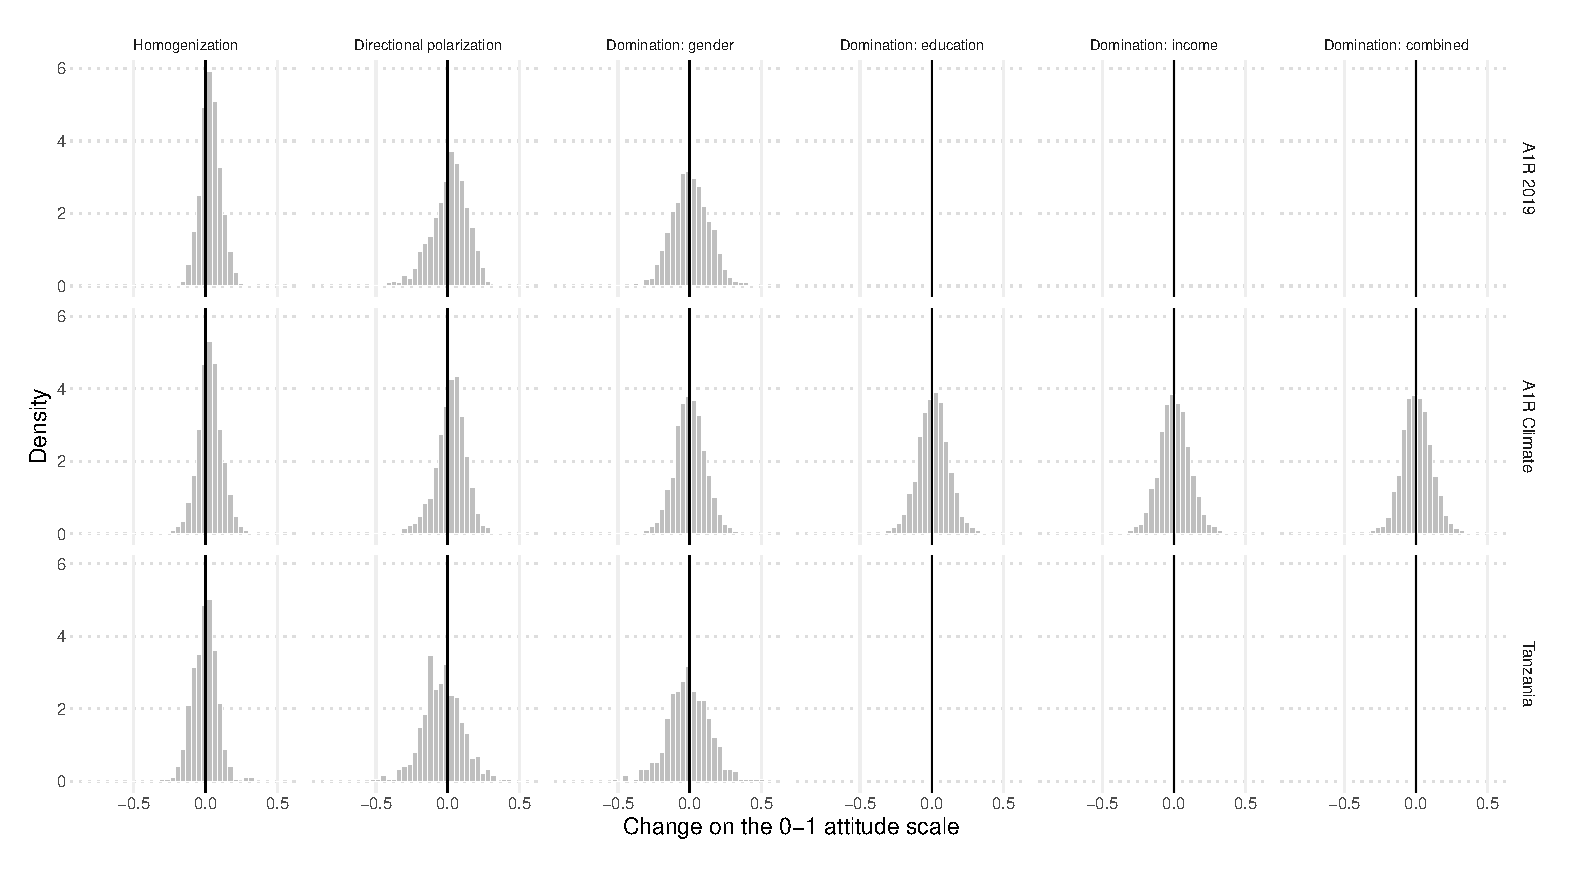
\includegraphics[width=.96\linewidth]{figs/dp_distributions.pdf}
\caption{Distributions of available-wave H, P and D in the new Deliberative Polls.
Bars are histograms of eligible group-item episodes, normalized to density within
each panel; vertical lines mark zero. Axes are shared. Empty panels indicate no
eligible demographic comparison. Items and groups within a poll are dependent;
these distributions are descriptive, not sampling distributions.}
\label{fig:dp}
\end{figure}
\end{landscape}

\begin{figure}[p]
\centering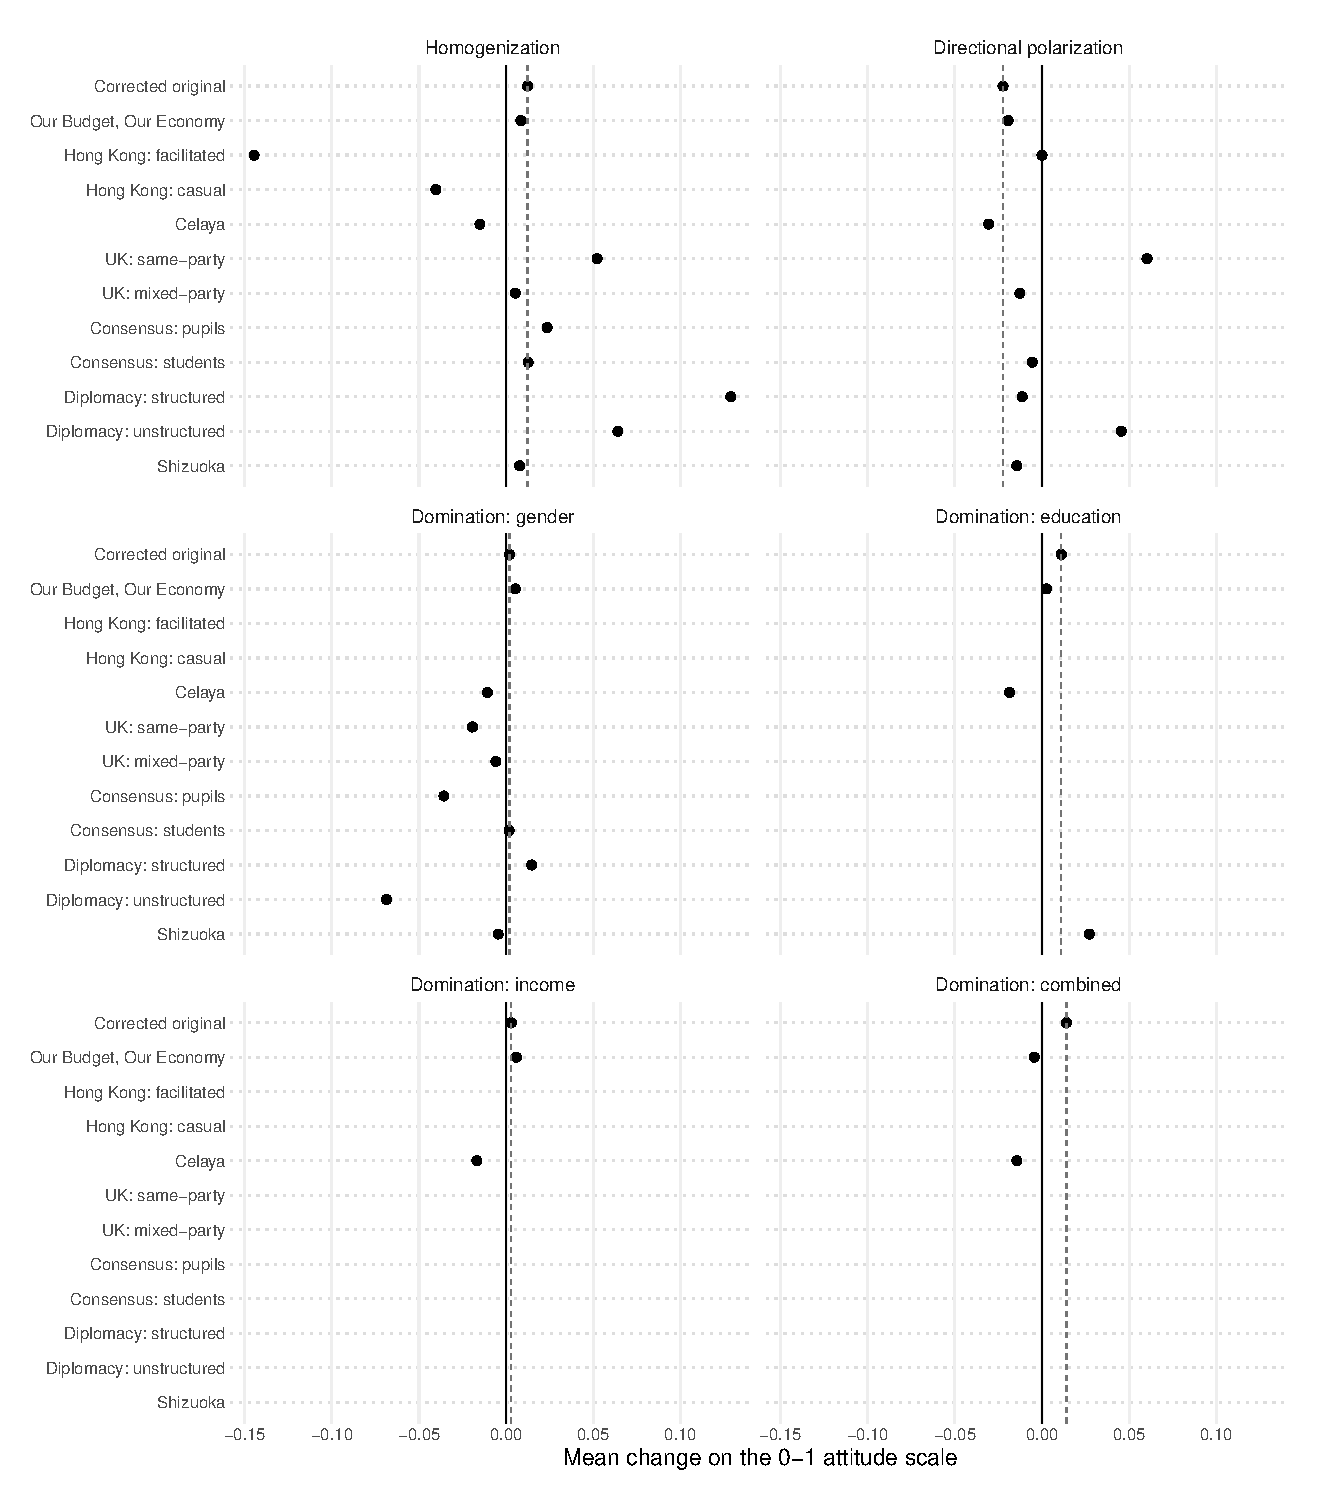
\includegraphics[width=\linewidth,height=.83\textheight,keepaspectratio]{figs/means_policy.pdf}
\caption{Paired policy estimates in the corrected original and other discussion designs.
Points are signed means across eligible group-item episodes; dashed lines are the
corrected original's paired benchmark for each measure. Conditions and study labels
identify the observed settings, not randomized cross-study treatment contrasts.
Points have no inferential intervals because these are descriptive study summaries.
The original measures indices and the extension measures individual items.}
\label{fig:means}
\end{figure}

The distinction between polarization definitions changes some apparent conclusions.
In Shizuoka, directional P is \policy{shizuoka}{p}, while absolute-distance P is
\policy{shizuoka}{p_absolute}. OBOE similarly gives \policy{ourbudgetoureconomy}{p}
and \policy{ourbudgetoureconomy}{p_absolute}. A negative directional mean does not
by itself establish movement closer to neutrality. Appendix~\ref{app:sensitivity}
reports both definitions and their eligible counts.

\subsection{Parsing domination}
The subgroup comparisons use paired responses throughout, so that composition is fixed and the weighted identity holds. Whole-group D varies across settings. The original's
positive education benchmark, \policy{correctedoriginal}{d_education}, is
\policy{a1rclimate}{d_education} in A1R Climate,
\policy{ourbudgetoureconomy}{d_education} in OBOE,
\policy{celaya}{d_education} in Celaya and
\policy{shizuoka}{d_education} in Shizuoka. These contrasts concern movement toward
initial subgroup positions. They are not direct measurements of power or persuasion.

Table~\ref{tab:components} separates the components. In the corrected original,
the disadvantaged education subgroup's mean movement is
\component{correctedoriginal}{education}{ext_dis}, compared with
\component{correctedoriginal}{education}{ext_adv} for advantaged members in the
same signed direction. In A1R Climate the corresponding means are
\component{a1rclimate}{education}{ext_dis} and
\component{a1rclimate}{education}{ext_adv}.
The disadvantaged component is positive and the advantaged component negative in
each OOS study with education data. Their directions therefore recur even though
the sign of whole-group D does not. These are signed movements toward initial
positions; midpoint or subgroup-reference crossings can complicate descriptions
of the final distance between subgroups.

\begin{table}[p]
\centering\small
\caption{Parsing domination: whole-group and subgroup movement}
\label{tab:components}
\textit{Gender}\par
\begin{tabular}{lrrr}
\toprule
Study / condition & Whole group D & Disadvantaged M & Advantaged M\\
\midrule
Corrected original & 0.002 / 46.3 (2433) & 0.039 / 55.9 (2434) & -0.035 / 35.9 (2434)\\
A1R 2019 & 0.007 / 50.2 (1853) & 0.051 / 57.4 (1853) & -0.035 / 38.3 (1853)\\
Our Budget, Our Economy & 0.005 / 43.2 (969) & 0.068 / 46.2 (969) & -0.052 / 25.6 (969)\\
Tanzania & -0.005 / 46.0 (517) & 0.074 / 65.8 (517) & -0.091 / 30.8 (517)\\
A1R Climate & 0.001 / 47.5 (6502) & 0.046 / 55.5 (6502) & -0.048 / 32.5 (6502)\\
\addlinespace
Celaya & -0.011 / 40.7 (54) & 0.034 / 51.9 (54) & -0.087 / 22.2 (54)\\
UK: same-party & -0.019 / 43.2 (162) & 0.013 / 42.6 (162) & -0.054 / 32.1 (162)\\
UK: mixed-party & -0.006 / 41.7 (156) & 0.027 / 50.0 (156) & -0.039 / 30.1 (156)\\
Consensus: pupils & -0.036 / 34.1 (41) & 0.025 / 34.1 (41) & -0.124 / 24.4 (41)\\
Consensus: students & 0.002 / 33.3 (24) & -0.010 / 29.2 (24) & -0.026 / 20.8 (24)\\
\addlinespace
Diplomacy: structured & 0.015 / 41.2 (17) & 0.118 / 47.1 (17) & -0.074 / 11.8 (17)\\
Diplomacy: unstructured & -0.069 / 11.8 (17) & -0.029 / 23.5 (17) & -0.125 / 11.8 (17)\\
Shizuoka & -0.005 / 40.4 (57) & 0.055 / 42.1 (57) & -0.064 / 24.6 (57)\\
\bottomrule
\end{tabular}
\par\medskip
\textit{Education}\par
\begin{tabular}{lrrr}
\toprule
Study / condition & Whole group D & Disadvantaged M & Advantaged M\\
\midrule
Corrected original & 0.011 / 51.2 (2383) & 0.052 / 58.5 (2385) & -0.028 / 39.5 (2385)\\
Our Budget, Our Economy & 0.003 / 44.6 (1493) & 0.047 / 45.9 (1493) & -0.052 / 25.6 (1493)\\
A1R Climate & 0.009 / 51.5 (5913) & 0.033 / 57.2 (5913) & -0.064 / 26.9 (5913)\\
Celaya & -0.019 / 32.7 (52) & 0.012 / 48.1 (52) & -0.110 / 13.5 (52)\\
Shizuoka & 0.027 / 52.0 (75) & 0.087 / 60.0 (75) & -0.049 / 29.3 (75)\\
\bottomrule
\end{tabular}
\par\medskip
\textit{Income}\par
\begin{tabular}{lrrr}
\toprule
Study / condition & Whole group D & Disadvantaged M & Advantaged M\\
\midrule
Corrected original & 0.003 / 50.0 (1135) & 0.052 / 55.8 (1135) & -0.033 / 39.6 (1135)\\
Our Budget, Our Economy & 0.006 / 44.1 (1486) & 0.060 / 45.1 (1486) & -0.054 / 26.1 (1486)\\
A1R Climate & 0.005 / 48.8 (6379) & 0.041 / 55.7 (6379) & -0.044 / 33.8 (6379)\\
Celaya & -0.017 / 35.8 (53) & 0.024 / 56.6 (53) & -0.073 / 15.1 (53)\\
\bottomrule
\end{tabular}
\par\medskip
\textit{Combined advantage}\par
\begin{tabular}{lrrr}
\toprule
Study / condition & Whole group D & Disadvantaged M & Advantaged M\\
\midrule
Corrected original & 0.014 / 52.2 (972) & 0.030 / 54.5 (972) & -0.062 / 30.8 (972)\\
Our Budget, Our Economy & -0.004 / 43.3 (397) & 0.021 / 45.6 (397) & -0.066 / 17.4 (397)\\
A1R Climate & 0.006 / 49.1 (3659) & 0.024 / 54.6 (3659) & -0.084 / 23.5 (3659)\\
Celaya & -0.014 / 36.7 (30) & -0.004 / 40.0 (30) & -0.108 / 16.7 (30)\\
\bottomrule
\end{tabular}

\begin{minipage}{\linewidth}\footnotesize
Cells report mean / percentage positive (eligible group-item episodes).
All samples are paired; each component retains its own defined direction and
available means. Positive disadvantaged M means movement toward the advantaged
initial mean. Negative advantaged M means movement toward the disadvantaged
initial mean. The within-cell weighted decomposition is exact; separately
averaged components need not reproduce average D. All estimates are descriptive.
\end{minipage}
\end{table}

\subsection{Attitude change}
Small H, P or D need not mean respondents barely changed their views. We parallel
the original paper's net/gross comparison using complete respondent pairs.
Net change is the absolute mean individual change within a group-item episode;
gross change is the mean absolute individual change. Opposing individual movements
can cancel in the former. Table~\ref{tab:change} averages each quantity across
eligible group-item episodes. The companion CSV also averages episodes equally
after aggregating their items, matching the original's alternative weighting.

\begin{table}[p]
\centering\small
\caption{Absolute net and gross attitude change on policy items}
\label{tab:change}

\begin{tabular}{lrrr}
\toprule
Study & Net & Gross & Pairs\\
\midrule
Corrected original & 0.089 & 0.203 & 2480\\
A1R 2019 & 0.102 & 0.200 & 1880\\
Our Budget, Our Economy & 0.116 & 0.186 & 1986\\
Hong Kong: facilitated & 0.000 & 0.133 & 1\\
Hong Kong: casual & 0.033 & 0.067 & 1\\
\addlinespace
Tanzania & 0.115 & 0.348 & 525\\
A1R Climate & 0.085 & 0.170 & 6825\\
Celaya & 0.054 & 0.256 & 56\\
UK: same-party & 0.087 & 0.131 & 188\\
UK: mixed-party & 0.064 & 0.125 & 160\\
\addlinespace
Consensus: pupils & 0.115 & 0.148 & 56\\
Consensus: students & 0.060 & 0.080 & 82\\
Diplomacy: structured & 0.127 & 0.157 & 27\\
Diplomacy: unstructured & 0.104 & 0.158 & 28\\
Shizuoka & 0.106 & 0.198 & 80\\
\bottomrule
\end{tabular}

\begin{minipage}{\linewidth}\footnotesize
All quantities use paired respondents on the 0--1 instrument scale. Net is the
absolute mean respondent change within a group-item episode; gross is the mean
absolute respondent change. Both columns then weight group-item episodes equally.
The original row uses its policy indices. Pairs counts episodes with at least one
complete respondent. These descriptive summaries do not identify why people changed.
\end{minipage}
\end{table}

\section{What replicates, and what remains open}
The evidence separates three questions that are easy to combine. First, do unused
Deliberative Polls reproduce the original signed averages? Not uniformly: the new
polls differ in directional polarization and one differs in homogenization.
Second, do other discussion formats show the same averages? Their descriptive
results also vary, with substantial differences in who participates, which topics
are discussed, group size, timing and measurement. A contrast between two rows
cannot isolate the effect of facilitation, composition, mode or any other design feature.

Third, does the distinction between whole-group and subgroup movement matter
outside the original study? The education decomposition indicates that it does.
A whole-group mean close to zero can accompany larger subgroup movements in opposing
signed directions. Reporting only D would omit that pattern. It would also leave
unanswered whether limited net movement merely reflects limited individual change,
which is why the gross-change comparison is part of the parallel analysis.

The present study is an analysis of observed pre/post discussions, including
selected treatment or conversation-completer samples. Some source experiments
contain randomized contrasts that are not estimated here. Such within-study
contrasts could address narrower causal questions, provided their assignment,
attrition, outcome and dependence structures are carried through explicitly.
They would answer a different question from pooling unrelated formats into a
single regression.

The remaining data work is concrete. Several public datasets need discussion-group
linkage; others require access to participant files or a verified baseline
instrument. The current search does not justify a claim about the universe of
all deliberative studies. Expanding the usable corpus and harmonizing original
indices with new items could change both the comparison and its precision.

\clearpage
\bibliographystyle{plainnat}
\bibliography{references}

\clearpage\appendix
\section{Sources, instruments and eligibility}
\begin{table}[htbp]
\centering\small
\caption{Public archives used in this analysis}\label{tab:sources}

\begin{tabular}{lll}
\toprule
Study & Archive & Released\\
\midrule
A1R 2019 & 10.7910/DVN/KJ8IH2 & 2021-07-27\\
Our Budget, Our Economy & 10.7910/DVN/XDDN2Y & 2019-09-10\\
Hong Kong & 10.7910/DVN/W9DAQM & 2021-10-26\\
Tanzania & 10.7910/DVN/S3NRQL & 2022-09-27\\
A1R Climate & 10.7910/DVN/IIOG1S & 2024-11-25\\
\addlinespace
Celaya & 10.7910/DVN/OOMED8 & 2019-05-15\\
UK partisan discussion & 10.7910/DVN/BM2A1Q & 2023-12-01\\
WhatsApp India & 10.7910/DVN/WYXEXN & 2026-01-04\\
US cross-party conversation & 10.7910/DVN/EVRMBG & 2023-11-14\\
Consensus: pupils & 10.34894/6IOPCF & 2023-12-13\\
\addlinespace
Consensus: students & 10.34894/6IOPCF & 2023-12-13\\
Diplomacy lab & 10.34894/SAZIAE & 2022-04-14\\
Shizuoka & 10.6084/m9.figshare.22229794 & 2023-03-07\\
\bottomrule
\end{tabular}

\end{table}
The accompanying \texttt{items.csv} is the item-level appendix: it records the
released labels, pre/post columns, instrument endpoints, missing codes, neutral
midpoint, construct and episode. It should be read with the linked source
instruments; not every archive label is verbatim questionnaire wording.
\texttt{events.csv} records study, condition, country, mode, date precision,
post timing and dependence family. \texttt{source\_register.csv} records the
specific evidence and unresolved requirements for included and deferred studies.
Source downloads are checked against the SHA-256 hashes in \texttt{files.csv}.

Harmonization does not convert rankings or nominal task choices into cardinal
attitudes. The pupil consensus study retains its fractional seven-point responses,
but supplies no P because a neutral midpoint label is unverified. Shizuoka's
procedural preferences and information belief remain separate. Climate policy,
concern and belief items are separate, as are affect and stereotypes in the
conversation studies. No public table number is substituted for missing respondent
microdata or discussion assignments.

The original's conceptual Figures 1--2 illustrate definitions and theoretical
expectations. They do not have new empirical observations to reproduce here.
Equations in this manuscript supply the definitions; the empirical distribution
figures parallel the original's Figure 3. Its Tables 1--3 correspond to our inventory,
magnitude/occurrence table and subgroup decomposition.

\section{Sampling and measurement sensitivity}\label{app:sensitivity}
\begin{landscape}
\begin{table}[p]
\centering\small
\caption{Full available-wave comparison and extension sampling sensitivity}

\begin{tabular}{lrrrrrr}
\toprule
Study / condition & H & P & Gender D & Education D & Income D & Combined D\\
\midrule
Corrected original & 0.013 / 58.6 & -0.022 / 44.0 & 0.002 / 47.1 & 0.010 / 52.3 & 0.002 / 50.5 & 0.013 / 51.9\\
A1R 2019 & 0.035 / 69.9 & 0.013 / 59.0 & 0.006 / 50.5 & -- & -- & --\\
Our Budget, Our Economy & 0.017 / 51.1 & -0.017 / 46.5 & 0.008 / 49.1 & 0.005 / 50.1 & 0.010 / 49.3 & 0.012 / 50.4\\
Hong Kong: facilitated & -0.145 / 0.0 & 0.000 / 0.0 & -- & -- & -- & --\\
Hong Kong: casual & -0.040 / 0.0 & -- & -- & -- & -- & --\\
\addlinespace
Tanzania & -0.006 / 48.6 & -0.037 / 37.2 & -0.008 / 45.3 & -- & -- & --\\
A1R Climate & 0.030 / 65.3 & 0.022 / 61.2 & 0.001 / 48.8 & 0.010 / 52.8 & 0.005 / 49.7 & 0.006 / 50.4\\
Celaya & -0.015 / 33.9 & -0.031 / 28.3 & -0.011 / 40.7 & -0.019 / 32.7 & -0.017 / 35.8 & -0.014 / 36.7\\
UK: same-party & 0.050 / 74.5 & 0.059 / 75.0 & -0.022 / 44.8 & -- & -- & --\\
UK: mixed-party & 0.004 / 53.1 & -0.016 / 38.9 & -0.009 / 40.4 & -- & -- & --\\
\addlinespace
Consensus: pupils & 0.024 / 55.4 & -- & -0.036 / 34.1 & -- & -- & --\\
Consensus: students & 0.013 / 28.0 & -0.006 / 23.0 & 0.002 / 33.3 & -- & -- & --\\
Diplomacy: structured & 0.129 / 74.1 & -0.011 / 31.8 & 0.015 / 41.2 & -- & -- & --\\
Diplomacy: unstructured & 0.064 / 57.1 & 0.045 / 40.9 & -0.069 / 11.8 & -- & -- & --\\
Shizuoka & 0.007 / 50.0 & -0.016 / 41.0 & -0.006 / 40.4 & 0.027 / 52.0 & -- & --\\
\bottomrule
\end{tabular}

\begin{minipage}{.95\linewidth}\footnotesize
Cells report mean / percentage positive using all observed respondents at each
wave. The DP and original entries reproduce Panel A of Table~\ref{tab:main};
the extension entries are a sampling sensitivity relative to its paired Panel B.
Differences can reflect changing respondent composition. Scale and missing-value
conventions are unchanged.
\end{minipage}
\end{table}
\end{landscape}

\begin{table}[p]
\centering\small
\caption{Directional and absolute-distance polarization}

\begin{tabular}{lrrrr}
\toprule
Study / condition & Directional P & Absolute P & N directional & N absolute\\
\midrule
Corrected original & -0.022 & 0.008 & 2434 & 2480\\
A1R 2019 & 0.014 & 0.047 & 1854 & 1880\\
Our Budget, Our Economy & -0.019 & 0.028 & 1827 & 1986\\
Hong Kong: facilitated & 0.000 & 0.000 & 1 & 1\\
Hong Kong: casual & -- & 0.033 & 0 & 1\\
\addlinespace
Tanzania & -0.038 & -0.008 & 520 & 525\\
A1R Climate & 0.024 & 0.039 & 6726 & 6825\\
Celaya & -0.031 & -0.013 & 53 & 56\\
UK: same-party & 0.060 & 0.061 & 188 & 188\\
UK: mixed-party & -0.013 & 0.015 & 149 & 160\\
\addlinespace
Consensus: pupils & -- & -- & 0 & 0\\
Consensus: students & -0.006 & 0.024 & 74 & 82\\
Diplomacy: structured & -0.011 & 0.052 & 22 & 27\\
Diplomacy: unstructured & 0.045 & 0.080 & 22 & 28\\
Shizuoka & -0.014 & 0.009 & 78 & 80\\
\bottomrule
\end{tabular}

\begin{minipage}{\linewidth}\footnotesize
Paired policy estimates. An initial midpoint makes directional P undefined but
leaves absolute-distance P defined. Midpoint crossings can produce opposite signs.
Counts are eligible group-item episodes and can differ between definitions.
\end{minipage}
\end{table}
\begin{figure}[p]
\centering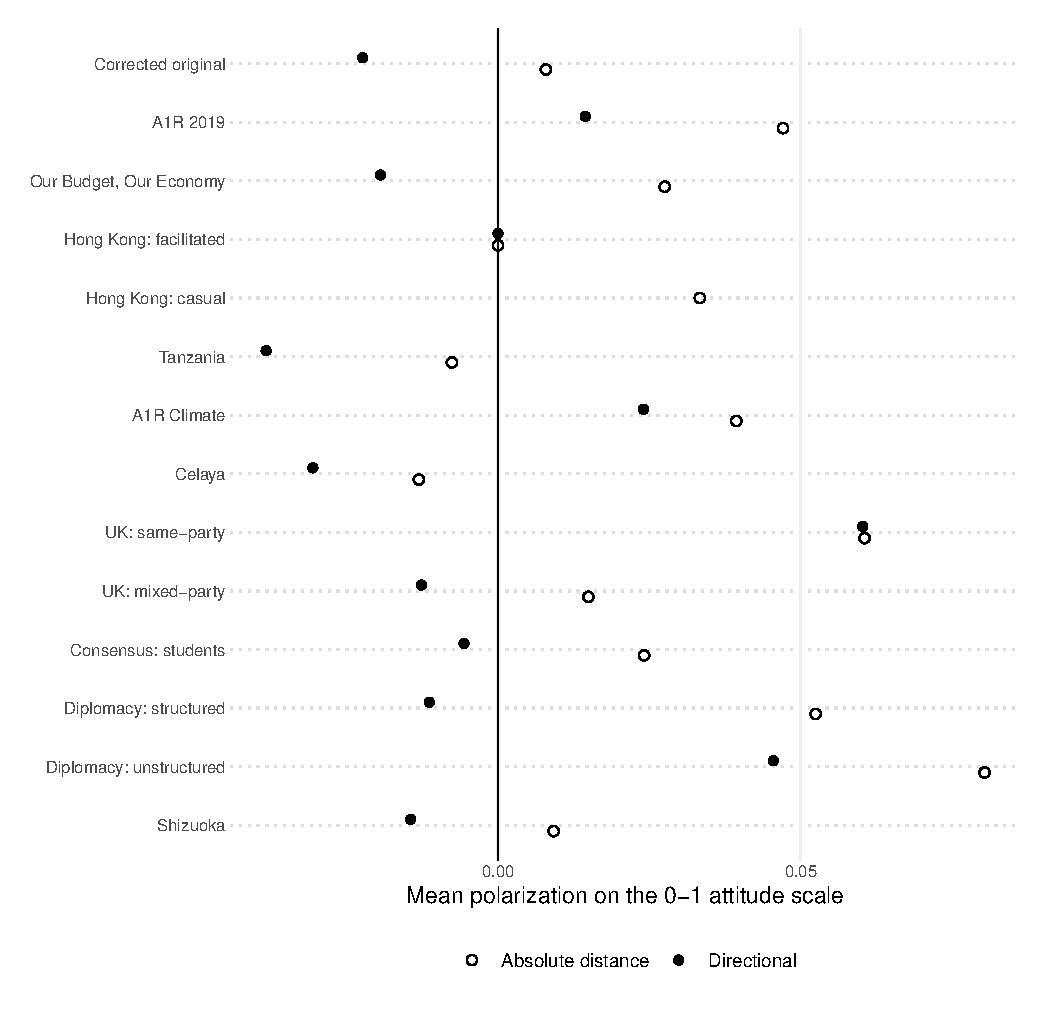
\includegraphics[width=.95\linewidth]{figs/polarization_definitions.pdf}
\caption{Two definitions of polarization on paired policy responses.
Each point is a study-condition mean. Directional and absolute-distance estimates
can use different eligible cells, as reported in the preceding table. These are
descriptive comparisons; zero marks no average movement under each definition.}
\end{figure}

The minimum-five restriction, event/family weights and leave-family-out results
are regenerated in \texttt{tabs/}. The restriction intentionally removes dyads and
triads from H/P comparisons; it is not a robustness test on an unchanged target
population. The WhatsApp source flags possible duplicates or associates, rather
than establishing duplicate identities. Its primary sample retains them, and a
separate sensitivity excludes flagged respondents using the same score definitions.

The correlation counterpart to the original's text analysis is
\texttt{paper\_correlations.csv}, computed separately by study-condition and
construct with pairwise eligible cells. \texttt{paper\_composition.csv} parallels
its regressions on disadvantaged share using paired policy samples. Those fits
are descriptive within-study associations. Predictions at shares 0.2 and 0.8
are retained only when inside the observed share range. They do not extrapolate
across unrelated discussion formats, and no independent-pair standard errors
are reported.

\section{Distributions across discussion designs}
\begin{figure}[p]
\centering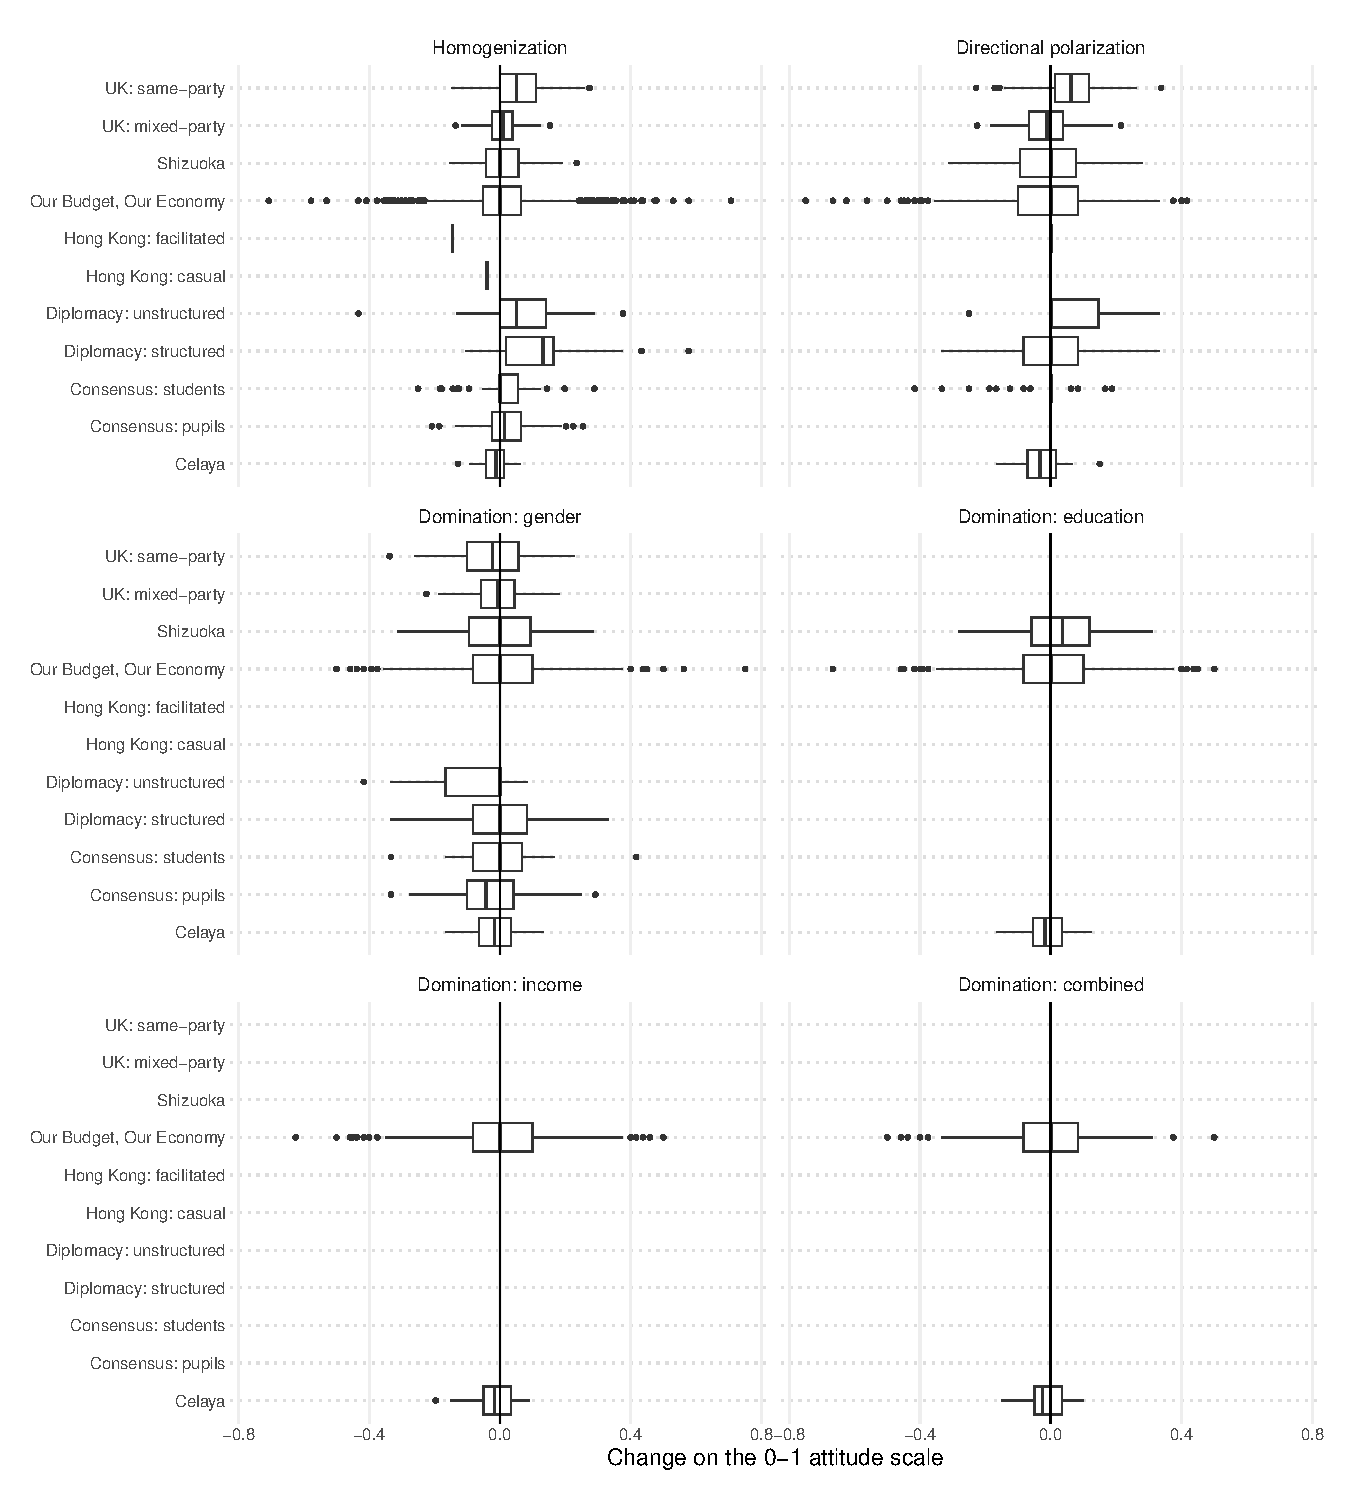
\includegraphics[width=\linewidth,height=.84\textheight,keepaspectratio]{figs/extension_distributions.pdf}
\caption{Distributions in the non-DP policy discussions.
Boxplots show medians, interquartile ranges, whiskers extending to 1.5 times the
interquartile range and observations beyond the whiskers. They summarize eligible
paired group-item episodes within each condition; their spread is not uncertainty
about the condition mean. Scales are shared across measures.}
\end{figure}
\begin{figure}[p]
\centering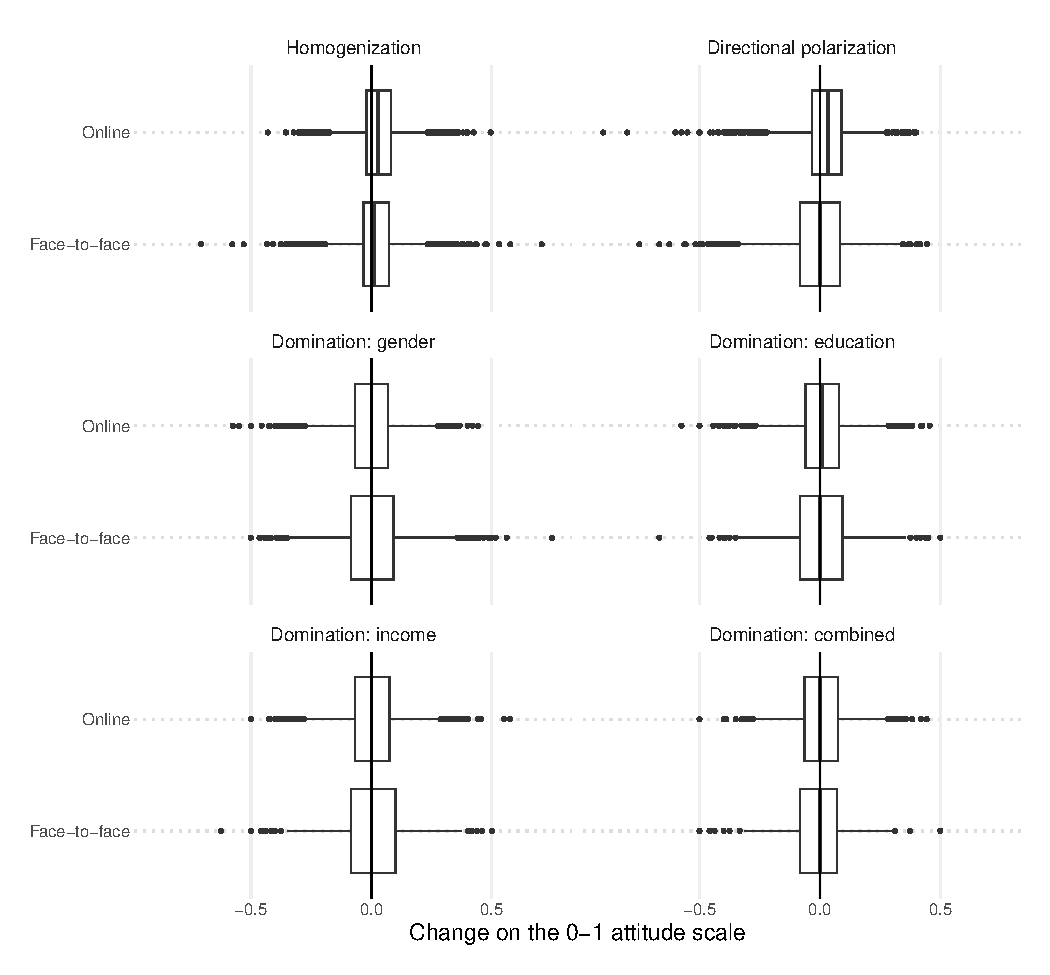
\includegraphics[width=\linewidth]{figs/distributions_mode.pdf}
\caption{Descriptive mode split, paralleling the original supplement.
Paired policy group-item episodes are grouped by the mode of their actual discussion.
Mode is confounded with study, topics, group size and participant selection.
Boxplots are episode distributions, not causal mode comparisons or confidence intervals.}
\end{figure}
\begin{figure}[p]
\centering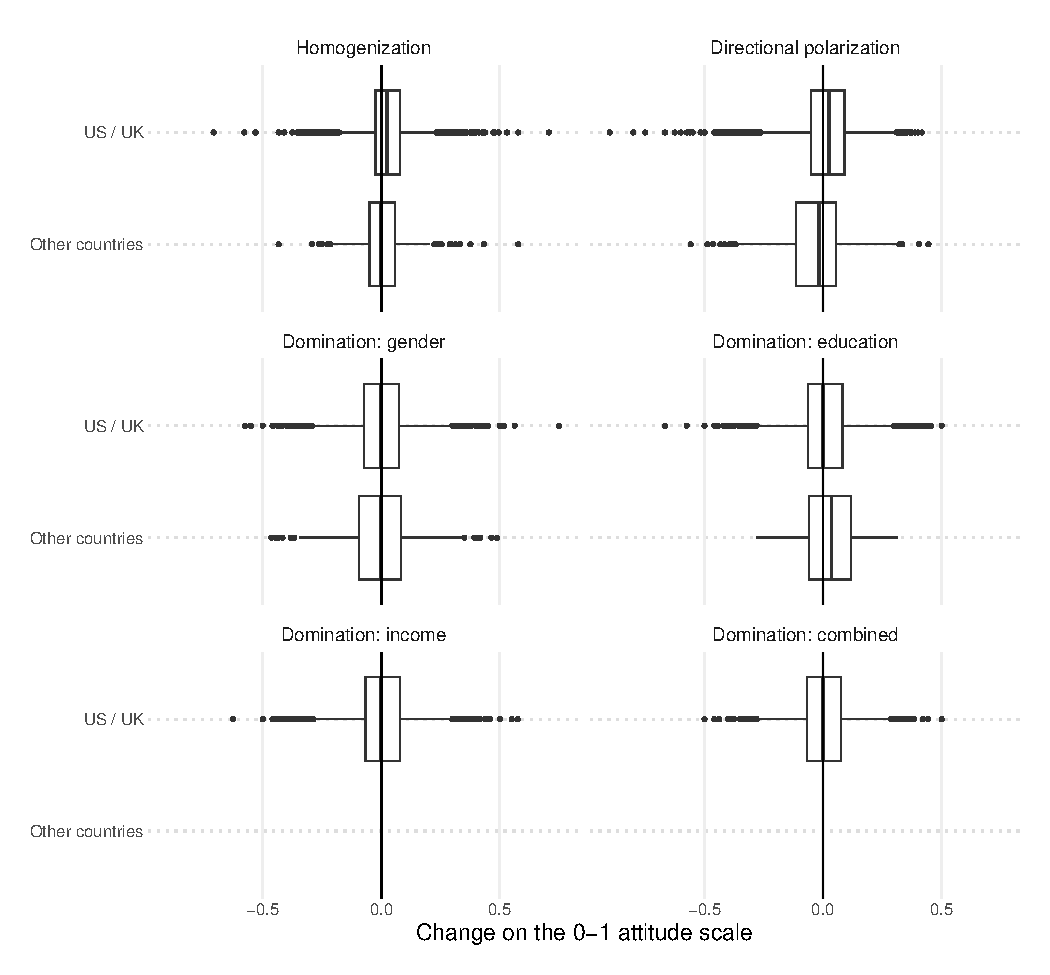
\includegraphics[width=\linewidth]{figs/distributions_region.pdf}
\caption{Descriptive country split, paralleling the original supplement.
Paired policy group-item episodes from US/UK studies are compared with the remaining
countries. The contributing studies and demographic coverage differ; boxplot spread
is not sampling uncertainty and the comparison does not isolate a country effect.}
\end{figure}

\clearpage
\section{Other outcome constructs}
Affective ratings, beliefs, environmental concern and social or stereotype judgments
are displayed separately below. They retain the same movement formulas but do not
share a substantive estimand merely because their scales can be rescaled to $[0,1]$.
In particular, affective P is not a partisan or religious affect gap.
\begin{landscape}
\begin{table}[p]\centering\small
\caption{Affective ratings: paired magnitudes and occurrence}

\begin{tabular}{lrrrrrr}
\toprule
Study / condition & H & P & Gender D & Education D & Income D & Combined D\\
\midrule
WhatsApp: gen\_HH & 0.015 / 33.2 & -0.068 / 19.6 & -- & 0.003 / 35.3 & 0.014 / 36.2 & 0.000 / 34.0\\
WhatsApp: gen\_HM & 0.009 / 32.7 & -0.081 / 18.6 & -- & 0.009 / 37.7 & 0.028 / 39.9 & 0.041 / 44.3\\
WhatsApp: igr\_HH & 0.013 / 33.3 & -0.087 / 17.1 & -- & 0.008 / 37.1 & -0.000 / 35.2 & -0.008 / 37.5\\
WhatsApp: igr\_HM & 0.016 / 32.9 & -0.086 / 16.6 & -- & -0.032 / 27.1 & 0.021 / 39.6 & 0.014 / 36.5\\
US cross-party conversation & 0.019 / 48.7 & -0.015 / 42.8 & -0.003 / 42.9 & -- & -- & --\\
\bottomrule
\end{tabular}

\par\footnotesize Cells are mean / percentage positive, as in Table~\ref{tab:main}.
WhatsApp gen/igr indicate general political/intergroup prompts; HH/HM indicate
Hindu--Hindu/Hindu--Muslim dyads. All four conditions share one study family.
\end{table}
\begin{table}[p]\centering\small
\caption{Beliefs, environmental concern and social judgments}
\textit{Beliefs}\par
\begin{tabular}{lrrrrrr}
\toprule
Study / condition & H & P & Gender D & Education D & Income D & Combined D\\
\midrule
Shizuoka & 0.021 / 50.0 & 0.028 / 57.1 & -0.049 / 20.0 & -0.016 / 37.5 & -- & --\\
\bottomrule
\end{tabular}
\par\medskip
\textit{Climate beliefs}\par
\begin{tabular}{lrrrrrr}
\toprule
Study / condition & H & P & Gender D & Education D & Income D & Combined D\\
\midrule
A1R Climate & 0.044 / 73.3 & 0.045 / 72.8 & 0.001 / 42.3 & 0.019 / 55.3 & 0.010 / 51.3 & 0.013 / 52.2\\
\bottomrule
\end{tabular}
\par\medskip
\textit{Environmental concern}\par
\begin{tabular}{lrrrrrr}
\toprule
Study / condition & H & P & Gender D & Education D & Income D & Combined D\\
\midrule
A1R Climate & 0.033 / 68.6 & 0.034 / 68.7 & -0.003 / 46.8 & 0.020 / 61.1 & 0.013 / 53.7 & 0.009 / 51.4\\
\bottomrule
\end{tabular}
\par\medskip
\textit{Social judgments}\par\input{tabs/paper_table_2_social_judgment_paired.tex}\par\medskip
\textit{Stereotype judgments}\par
\begin{tabular}{lrrrrrr}
\toprule
Study / condition & H & P & Gender D & Education D & Income D & Combined D\\
\midrule
WhatsApp: gen\_HH & -0.001 / 29.9 & -- & -- & -0.013 / 32.3 & -0.001 / 33.2 & -0.013 / 29.4\\
WhatsApp: gen\_HM & 0.026 / 33.8 & -- & -- & -0.009 / 37.2 & 0.019 / 35.5 & 0.008 / 36.4\\
WhatsApp: igr\_HH & -0.002 / 29.6 & -- & -- & -0.025 / 26.8 & -0.021 / 26.8 & 0.031 / 33.3\\
WhatsApp: igr\_HM & 0.011 / 30.8 & -- & -- & -0.027 / 26.2 & 0.001 / 31.5 & 0.011 / 38.3\\
\bottomrule
\end{tabular}

\par\footnotesize Cells are mean / percentage positive; constructs are not pooled.
\end{table}
\end{landscape}
\begin{figure}[p]\centering
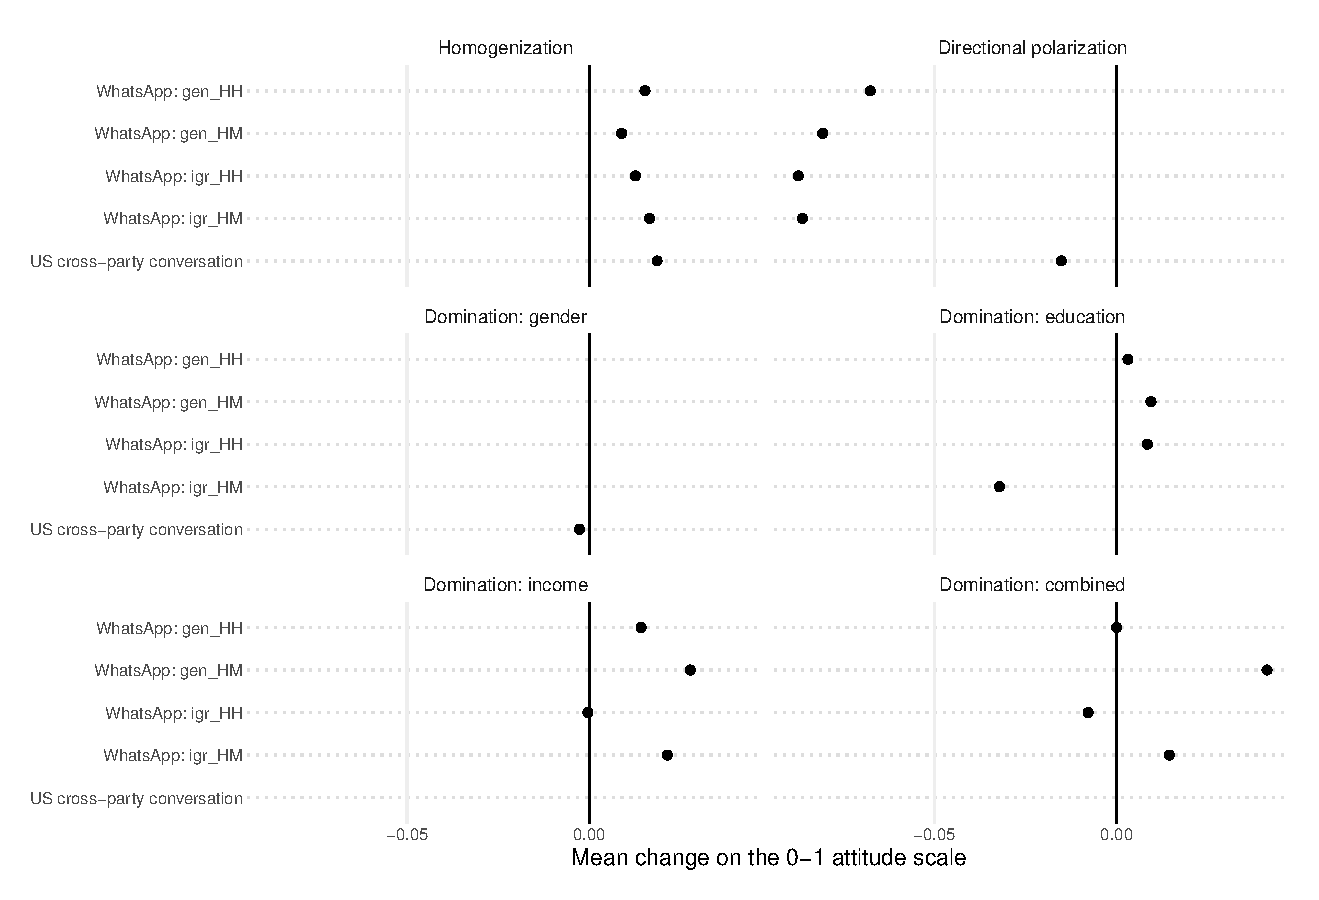
\includegraphics[width=\linewidth]{figs/means_affect.pdf}
\caption{Affective-rating means by observed discussion condition. Points are descriptive
paired group-item means, not effects on an in-party/out-party affect gap. Missing
panels have no eligible demographic comparison.}
\end{figure}
\clearpage
\section{Exploratory comparisons within studies}
Exposure to opposing views is one possible explanation to examine, rather than
assuming that the DP label itself determines outcomes. The UK experiment varies
partisan composition and can inform that hypothesis. Diplomacy varies discussion
structure among participants already selected for disagreement; it cannot isolate
the effect of exposure. Hong Kong varies facilitation and information in only two
groups. The all-study comparison does not identify these mechanisms. We therefore
treat the following contrasts as exploratory. A correlation between initial
dispersion and subsequent H would also be partly mechanical because initial
dispersion is a component of H; it would not establish an exposure effect.

Table~\ref{tab:design} puts two comparisons on a 0--100 scale. In the UK study,
mixed-party groups exhibit much less directional and absolute polarization than
same-party groups. Their mean gender D is also closer to zero, although both signs
are negative. Same-party groups homogenize substantially more. Thus less
polarization and more agreement do not rank the conditions in the same order.
In the Diplomacy experiment, structured discussions have greater homogenization,
less polarization on both definitions, and gender D closer to zero than
unstructured discussions. These are favorable descriptive patterns if lower
extremity and less demographic-directional movement are the criteria; neither
agreement nor movement toward neutrality is itself a measure of decision quality.

\begin{table}[htbp]
\centering\small
\caption{Discussion conditions compared on a 0--100 attitude scale}
\label{tab:design}

\begin{tabular}{lrrrr}
\toprule
Study / condition & H & Directional P & Absolute P & Gender D\\
\midrule
Corrected original & 1.23 & -2.24 & 0.79 & 0.19\\
UK: same-party & 5.21 & 6.02 & 6.05 & -1.93\\
UK: mixed-party & 0.52 & -1.27 & 1.49 & -0.60\\
Diplomacy: structured & 12.88 & -1.14 & 5.25 & 1.47\\
Diplomacy: unstructured & 6.41 & 4.55 & 8.04 & -6.86\\
\bottomrule
\end{tabular}

\begin{minipage}{\linewidth}\footnotesize
Paired policy ratings; equal weights for eligible group-item episodes. Positive H
means lower within-group dispersion. Positive P means greater extremity under the
indicated definition. Positive gender D means movement along the initial
disadvantaged-to-advantaged direction; it is not a direct measure of influence.
The UK conditions comprise 345 people in 47 same-party groups and 308 in 40
mixed-party groups. The same 105 people in 35 Diplomacy triads experience both
conditions on different topics. Eligible counts vary by measure; gender D uses
162/156 group-items in the UK and 17/17 in Diplomacy. CSV output supplies all counts.
The original uses policy indices, whereas the extensions use individual items.
\end{minipage}
\end{table}

These summaries do not exploit either study's assignment design to estimate a
causal contrast. The UK comparison conditions on observed discussion participation
and combines the crossed affect-prime treatments; a design-based analysis would
also address baseline timing and attrition. Diplomacy requires within-triad
contrasts accounting for topic, randomized order and possible carryover. Its
topics were selected for disagreement, and demographic comparisons are limited
to gender. The current estimates therefore support a description of these samples,
not a general ranking of deliberative formats or a test that DPs outperform them.

\end{document}
